% Use the base layout without conference or publication branding.
\PassOptionsToPackage{capitalise,noabbrev}{cleveref}
\PassOptionsToPackage{hypertexnames=false}{hyperref}
\documentclass[12pt,cleveref]{jmlr}

\usepackage{times}
\usepackage{mathtools}
\usepackage{microtype}
\usepackage{tikz}
\usetikzlibrary{arrows.meta,calc,decorations.pathreplacing}
\usepackage{wrapfig}
\setlength{\marginparwidth}{1in}
\setlength{\marginparsep}{0.15in}
\usepackage{todonotes}
\usepackage{xurl}
\hypersetup{linkcolor=blue!55!black,citecolor=blue!55!black,urlcolor=blue!55!black}

% Keep named proofs while using the class's proof typography and QED mark.
\renewenvironment{proof}[1][\proofname]
{\par\noindent{\bfseries\upshape #1\ }}
{\jmlrQED}
\usepackage{thm-restate}
\usepackage{autonum} % load last

% Restore theorem link targets omitted by the class on recent LaTeX kernels.
\makeatletter
\let\ps@jmlrtps\ps@plain
\patchcmd{\@jmlrmaketitle}
{\jmlrpreauthor \ignorespaces\@author \jmlrpostauthor}
{\ifx\@author\@empty\vskip\aftermaketitskip\else\jmlrpreauthor \ignorespaces\@author \jmlrpostauthor\fi}
{}{\errmessage{Title layout patch failed}}
\ifdefined\MakeLinkTarget
\patchcmd{\@begintheorem}{\hskip\labelsep}{\MakeLinkTarget{\@currentcounter}\hskip\labelsep}{}{\errmessage{Theorem hyperlink patch failed}}
\patchcmd{\@opargbegintheorem}{\hskip\labelsep}{\MakeLinkTarget{\@currentcounter}\hskip\labelsep}{}{\errmessage{Named theorem hyperlink patch failed}}
\fi
\makeatother

\crefname{lemma}{Lemma}{Lemmas}
\crefname{proposition}{Proposition}{Propositions}
\crefname{equation}{Eq.}{Eqs.}
\Crefname{equation}{Eq.}{Eqs.}
\crefname{equality}{Eq.}{Eqs.}
\Crefname{equality}{Eq.}{Eqs.}
\crefname{inequality}{Ineq.}{Ineqs.}
\Crefname{inequality}{Ineq.}{Ineqs.}
\creflabelformat{equality}{\textup{(#2#1#3)}}
\creflabelformat{inequality}{\textup{(#2#1#3)}}
\crefrangelabelformat{equality}{\textup{(#3#1#4)--(#5#2#6)}}
\crefrangelabelformat{inequality}{\textup{(#3#1#4)--(#5#2#6)}}
% Equation labels record their cleveref type by name instead of through
% \label[type]{...}, whose optional argument is lost inside amsmath displays
% with TeX Live 2026.
\makeatletter
\newcommand{\eqlabel}[1]{\global\@namedef{advcvx@labeltype@#1}{equality}\label{#1}}
\newcommand{\ineqlabel}[1]{\global\@namedef{advcvx@labeltype@#1}{inequality}\label{#1}}
\AtBeginDocument{%
    \let\advcvx@label@noarg\label@noarg
    \def\label@noarg#1{%
        \@ifundefined{advcvx@labeltype@#1}%
        {\advcvx@label@noarg{#1}}%
    {\label@optarg[\csname advcvx@labeltype@#1\endcsname]{#1}}}%
}
\makeatother
\newcommand{\proofpart}[2]{%
    \par\addvspace{1.2\baselineskip}
    \noindent
    \textcolor{blue!55!black}{\rule[-0.2ex]{2pt}{1.25em}}%
    \hspace{0.6em}%
    {\sffamily\bfseries\color{blue!55!black}Part #1}%
    \hspace{0.8em}%
    {\sffamily\bfseries #2}%
    \par\nobreak\smallskip
    \noindent\ignorespaces
}
\newcommand{\proofstepinline}[1]{%
    \par\addvspace{0.6\baselineskip}
    \noindent
    {\normalfont\normalsize\bfseries\color{blue!55!black}Step #1.}\enspace\ignorespaces
}
\newcommand{\reason}[1]{\texttt{(#1)}}
\newcommand{\explan}[2]{\stackrel{\reason{#2}}{#1}}
\newcommand{\R}{\mathbb R}
\newcommand{\E}{\mathbb E}
\newcommand{\Pp}{\mathbb P}
\newcommand{\K}{\mathcal K}
\newcommand{\cP}{\mathcal P}
\newcommand{\F}{\mathcal F}
\newcommand{\N}{\mathcal N}
\newcommand{\T}{\mathcal T}
\newcommand{\tr}{\operatorname{tr}}
\newcommand{\Lip}{\operatorname{Lip}}
\newcommand{\op}{\mathrm{op}}
\newcommand{\Reg}{\operatorname{Reg}}
\newcommand{\eReg}{\operatorname{eReg}}
\newcommand{\qReg}{\operatorname{qReg}}
\newcommand{\argmin}{\operatornamewithlimits{arg\,min}}
\newcommand{\1}{\mathbf 1}
\newcommand{\eps}{\varepsilon}
\renewcommand{\epsilon}{\varepsilon}
\newcommand{\ip}[2]{\left\langle #1,#2\right\rangle}
\newcommand{\norm}[1]{\left\lVert #1\right\rVert}
\newcommand{\normm}[2]{\left\lVert #1\right\rVert_{#2}}
\newcommand{\alireza}[1]{\todo[color=blue!20,size=\tiny]{Alireza: #1}}
\newcommand{\tor}[1]{\todo[color=red!20,size=\tiny]{Tor: #1}}
\newcommand{\kevin}[1]{\todo[color=green!20,size=\tiny]{Kevin: #1}}

% Provisional title.
\title[Adversarial Bandit Convex Optimization]
{Adversarial Bandit Convex Optimization with \texorpdfstring{$d^{3/2}\sqrt{n}$}{d\^{}(3/2) sqrt(n)} Regret}
\author{}

\begin{document}
\maketitle

\begin{abstract}
    We study adversarial bandit convex optimization, where in each of $n$ rounds a learner chooses a point $A_t$ in a convex body $\K\subset\R^d$ and observes only a noisy value of a convex loss $f_t:\K\to[0,1]$ at that point. The losses are chosen by an adversary, who may change them from round to round and adapt them to the learner's past actions.
    We improve the best known regret bound for this problem from $\widetilde O(d^{5/2}\sqrt n)$ \citep{lattimore2020improved,lattimore2026bandit} to $\widetilde O(d^{3/2}\sqrt n)$, which matches the rate conjectured by \citet{bubeck2017kernel}.
    Together with the recent lower bound of $\Omega(d^{4/3}\sqrt n)$ due to
    \citet{rajaraman2026price}, it determines the minimax regret up to a
    factor of $d^{1/6}$ and logarithmic factors.
    The algorithm is an online Newton step with Gaussian exploration.
    Unlike earlier methods of this kind, it uses unbiased estimates of the
    gradient and Hessian of the Gaussian smoothing of the loss, rather than
    of an optimistic surrogate.
\end{abstract}

\section{Introduction}
\label{sec:introduction}
In adversarial bandit convex optimization, a learner plays against an adversary for $n$ rounds. In round $t$, the adversary chooses a convex loss $f_t:\K\to[0,1]$, which may depend on everything that happened in earlier rounds. The learner then chooses an action $A_t\in\K$ and observes $f_t(A_t)$ plus noise. The goal is small regret: the learner's cumulative loss should be close to that of the best fixed action in hindsight for the realized losses $f_1,\ldots,f_n$, as defined in \cref{eq:regret}. Apart from convexity and boundedness, we make no assumptions on the losses. In particular, they need not be smooth or strongly convex.

We present an algorithm whose regret is $\widetilde O(d^{3/2}\sqrt n)$ with high probability. In each round, the algorithm estimates a quadratic approximation of a Gaussian smoothing of the loss and runs an online Newton step on these quadratics, while keeping its mean inside a focus region where the approximation can be trusted. A restart rule fires only when the regret of the current epoch\tor{The meaning of `epoch' may be unclear here.} is already negative, so restarts do not add to the regret.

\section{Related Work}
\label{sec:related-work}
Early algorithms estimate the gradient of a smoothed loss from a single function value \citep{kleinberg2004nearly,flaxman2005online}. They are simple, but their regret grows faster than $\sqrt n$. \citet{hazan2016optimal} obtained the first $\widetilde O(\sqrt n)$ bound,\tor{The Hazan paper gives an actual algorithm. Slightly earlier Bubeck and Eldan gave a non-constructive $\sqrt{n}$ bound. And there is even earlier the $d = 1$ case} with exponential dependence on $d$, and \citet{bubeck2017kernel} gave the first polynomial-time algorithm with $\widetilde O(\operatorname{poly}(d)\sqrt n)$ regret. Since then the question has been the dependence on $d$. \citet{lattimore2020improved} showed that the minimax regret is $\widetilde O(d^{5/2}\sqrt n)$, without giving an algorithm. The online Newton method of \citet{fokkema2024online} has regret $\widetilde O(d^{7/2}\sqrt n)$, and \citet[Chapter~11]{lattimore2026bandit} reduces this to $\widetilde O(d^{5/2}\sqrt n)$. These methods build quadratic approximations of an optimistic surrogate of the loss, and between restarts they decay the inverse covariance. Our algorithm uses the ordinary Gaussian smoothing and needs no such modification. \Cref{thm:main} improves the best bound by a factor of $d$ and reaches the rate $d^{3/2}\sqrt n$ conjectured by \citet[Conjecture~1]{bubeck2017kernel}.
The same rate was known for stochastic losses \citep{fokkema2024online}. On the lower-bound side, \citet{rajaraman2026price} recently proved $\Omega(d^{4/3}\sqrt n)$, improving on the $\Omega(d\sqrt n)$ of \citet{dani2008stochastic}, which leaves a gap of $d^{1/6}$. We refer to \citet{lattimore2026bandit} for an overview of the literature on bandit convex optimization.

\section{Notation and Problem Formulation}
\label{sec:setting}

For $r>0$, let $\mathbb{B}_r=\{x\in\R^d:\norm{x}\leq r\}$ be the Euclidean ball
of radius $r$. Let $\K\subset\R^d$ be a convex body that is known to the
learner. An affine preprocessing step puts the body in the position
$\mathbb{B}_1\subseteq\K\subseteq\mathbb{B}_{2d}$.
\tor{reference needed and let's discuss this.}
\tor{at some point will you talk about how $\K$ is represented and the computation implications?}
In each round $t=1,\ldots,n$, an adversary chooses a convex loss
$f_t:\K\to[0,1]$, the learner chooses an action $A_t\in\K$, and it observes
$f_t(A_t)+\xi_t$, where $\xi_t$ is the noise in round $t$.
The adversary is adaptive: $f_t$ may depend on everything that happened
before round $t$, including the earlier actions of the learner, but not on
the randomness that the learner uses in round $t$.
To make this precise, let $\zeta_t$ be the randomness of the algorithm in
round $t$ which it uses to make decisions, let
$\F_t=\sigma(f_1,\zeta_1,\xi_1,\ldots,f_t,\zeta_t,\xi_t,f_{t+1})$, and let
$\E_t[\cdot]=\E[\cdot\mid\F_{t-1}]$ and $\Pp_t(\cdot)=\Pp(\cdot\mid\F_{t-1})$.\tor{At some point I decided that $\E_t=\E[\cdot\mid\F_t]$, which I think usually less ambiguous but does make the notation a bit less concise. I leave it to you though. People are inconsistent.}
Thus $\F_{t-1}$ contains the history up to the end of round $t-1$ together
with the loss $f_t$, so that under $\E_t$ the loss of round $t$ is fixed and
only the randomness of the learner and the noise in that round remain.
The noise is conditionally subgaussian, i.e., for all $t$,
\begin{align}
    \E_t[\xi_t\mid\zeta_t]=0,
    \qquad
    \E_t[\exp(\xi_t^2)\mid\zeta_t]\leq2.
    \eqlabel{eq:noise}
\end{align}
This includes noiseless feedback.
The quantity of interest is the realized regret against the best fixed
action in hindsight,
\begin{align}
    \Reg_n=\sum_{t=1}^nf_t(A_t)-\inf_{x\in\K}\sum_{t=1}^nf_t(x).
    \eqlabel{eq:regret}
\end{align}
Since the losses may react to the actions of the learner, the best action in
hindsight is itself random and depends on the whole game.
Let $\pi(x)=\inf\{r>0:x\in r\K\}$ be the Minkowski functional of $\K$.
The Minkowski projection onto $\K$ is the map from $\R^d$ to $\K$ given by
\begin{align}
    x\longmapsto\frac{x}{\max\{1,\pi(x)\}}.
\end{align}
It leaves points in $\K$ unchanged and maps each $x\notin\K$ to the point
where the segment from $0$ to $x$ meets the boundary of $\K$.
Let $U$ be uniform on the Euclidean unit sphere.
The only geometric quantity in the result is
\begin{align}
    M=\max\left\{\frac1{\sqrt d},\E[\pi(U)]\right\}.
    \eqlabel{eq:M}
\end{align}
The rounding $\mathbb{B}_1\subseteq\K$ implies that $\pi$ is $1$-Lipschitz,
and in particular $M\leq1$.
For a symmetric matrix $B\in\R^{d\times d}$, which need not be positive
semidefinite, we write $\normm{x}{B}^2=x^\top Bx$, and $\norm{B}_{\op}$ for
its operator norm.
Write $\gamma_{\mu,\Sigma}$ for the density of the multivariate normal
distribution $\N(\mu,\Sigma)$, for $\mu\in\R^d$ and $\Sigma\in\R^{d\times d}$
symmetric positive definite.
For a convex function $h:\R^d\to\R$ and points $x,y\in\R^d$ such that $h$ is
differentiable at $y$, the Bregman divergence of $h$ is
$D_h(x\,\|\,y)=h(x)-h(y)-\ip{\nabla h(y)}{x-y}$, which is nonnegative by convexity.
A convex function is differentiable almost everywhere, so $D_h(x\,\|\,X)$ is
defined almost surely when $X$ is Gaussian with a positive definite
covariance.

\paragraph{The Convex Extension.}
Each loss $f_t$ is defined only on $\K$, but the algorithm samples points from
Gaussian distributions, and these can fall outside $\K$.
Following \citet{fokkema2024online} and \citet[Eq.~(10.6)]{lattimore2026bandit},
we work with a convex extension of $f_t$ to $\R^d$ whose value at
any point can be computed from a single value of $f_t$.
Fix $\eps\in(0,1/2]$, let $\K_\eps=(1-\eps)\K$, and define
\begin{align}
    \pi_\eps(x)
    &
    % =\max\left\{1,\frac{\pi(x)}{1-\eps}\right\}
    =
    \begin{cases}
        1               & \text{if }x\in\K_\eps, \\
        \frac{\pi(x)}{1-\eps} & \text{otherwise}\,,
    \end{cases}
    \quad\text{and}\quad v(x)=\pi_\eps(x)-1\,.
    \eqlabel{eq:extension-notation}
\end{align}
% Following \citet{fokkema2024online} and \citet[Eq.~(10.6)]{lattimore2026bandit},
Define for all $x\in\R^d$
\begin{align}
    e_t(x)
    =\pi_\eps(x)f_t\!\left(\frac{x}{\pi_\eps(x)}\right)
    +\frac{2}{\eps}v(x)\,.
    \eqlabel{eq:extension}
\end{align}

\begin{wrapfigure}{r}{0.46\textwidth}
    \vspace{-6pt}
    \centering
    % Editable TikZ source: figures/extension.tex. Rebuild with: make -C figures
    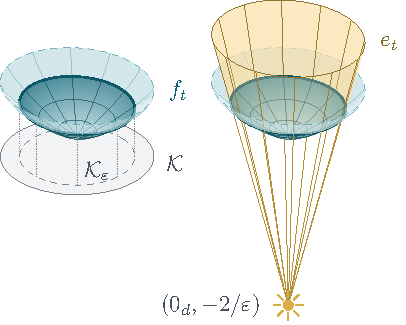
\includegraphics{figures/extension.pdf}
    \caption{\small Left: a convex loss $f_t:\K\to[0,1]$, with $\K$ the unit disc.
    Right: its extension $e_t:\R^d\to\R$.}
    \label{fig:extension}
    \vspace{-4pt}
\end{wrapfigure}
If $x\in\K_\eps$, then $\pi_\eps(x)=1$ and $v(x)=0$, so $e_t(x)=f_t(x)$.
If $x\notin\K_\eps$, then $x/\pi_\eps(x)$ lies on the boundary of
$\K_\eps$. Thus evaluating $e_t$ at any point of $\R^d$ requires only one
evaluation of $f_t$, at the point $x/\pi_\eps(x)\in\K_\eps$.
For $y\in\partial\K_\eps$ and $r\geq1$, the definition gives
$e_t(ry)=rf_t(y)+2(r-1)/\eps$. Hence the extension is affine along each
ray outside $\K_\eps$, as illustrated in \cref{fig:extension}.

The following lemma collects the properties used in the analysis.
\begin{lemma}\label{lem:extension}
    For $0<\eps\leq1/2$, the functions $e_t$ and $e_t-v/\eps$ are convex on
    $\R^d$, and $\Lip(e_t)\leq5/\eps$. Moreover, $e_t=f_t$ on $\K_\eps$ and
    \begin{align}
        f_t\bigl(x/\pi_\eps(x)\bigr)\leq e_t(x)
        \qquad\text{for every }x\in\R^d.
    \end{align}
\end{lemma}
The convexity statements follow from
\citet[Proposition~3.23]{lattimore2026bandit}. Appendix~\ref{app:extension}
gives the short argument and verifies the constant in the Lipschitz bound.

\section{The Algorithm}
\label{sec:algorithm}

There are three main ingredients in \textit{Smooth ONS} (\cref{alg:main}).
The first is \textit{Gaussian smoothing}:
the algorithm estimates the gradient and Hessian of a
smoothed version of the loss $e_t$, and forms a
quadratic model of the loss at the current mean $\mu_t$.
The second is \textit{online Newton step}:
the mean and covariance of the sampling distribution are updated
by an online Newton step on the quadratic model.
Third is \textit{focus region and restart}: the algorithm maintains an intersection
of ellipsoids called the \textit{focus region}.
The algorithm restarts with fresh parameters
when it certifies that it has done better than every action in
the \textit{focus region}.
The analysis shows that the regret accumulated before a restart is negative, so
the total regret is bounded by the regret accumulated after the last restart.
\begingroup
\RestyleAlgo{ruled}
\DontPrintSemicolon
\SetAlgoNoLine
\SetAlgoNoEnd
\LinesNumbered
\SetAlFnt{\small}
\newcommand{\algmark}[1]{\tikz[remember picture,overlay]\coordinate (#1);}
\newcommand{\algbrace}[3]{%
    \begin{tikzpicture}[remember picture,overlay]
        \draw[decorate,decoration={brace,amplitude=4pt},black!60]
        ([xshift=-64pt,yshift=7pt]ons-right |- #1) --
        ([xshift=-64pt,yshift=-5pt]ons-right |- #2)
        node[midway,right=7pt,text width=55pt,align=left,
        font=\scriptsize\itshape,text=black!65]{#3};
    \end{tikzpicture}%
}
\SetKwInput{KwIn}{Input}
\begin{algorithm2e}[!t]
    \caption{Smooth ONS}
    \label{alg:main}
    \KwIn{$\sigma$, $\eta$, $\lambda$, $R$, $\rho$ and $\eps$\hfill
    \algmark{ons-right}}
    \setlength{\rightskip}{70pt}
    \While{fewer than $n$ rounds have been played}{
        Start an epoch: set $\mu_1=0$, $\Sigma_1=\sigma^2I_d$, $K_0=\K_\eps$ and $Q_0=0$\;
        \For{$t=1,2,\ldots$ as long as rounds remain}{
            {\setlength{\rightskip}{0pt}%
            Set $E_t=\bigl\{x\in\R^d:\normm{x-\mu_t}{\Sigma_t^{-1}}^2\leq R^2\bigr\}$ and $K_t=K_{t-1}\cap E_t$\;}
            \algmark{ons-sample-top}Sample $X_t\sim\N(\mu_t,\Sigma_t)$ and play $A_t=X_t/\pi_\eps(X_t)$ and observe $f_t(A_t)+\xi_t$ %\kevin{We should call this $Y_t$ as equation (6) references it as $Y_t$} \;
            \algmark{ons-sample-bottom}Compute $g_t$ and $H_t$ by \cref{eq:gaussian-derivatives-estimates}\;
            \If{$\Sigma_t^{-1}+\eta\lambda H_t/2\not\succ0$}{play $0$ in all remaining rounds and stop\;}
            \algmark{ons-newton-top}Set $\Sigma_{t+1}^{-1}=\Sigma_t^{-1}+\eta\lambda H_t/2$\;
            \algmark{ons-newton-bottom}Set $\mu_{t+1}=\argmin_{u\in K_t} \normm{u-\bigl(\mu_t-\eta \Sigma_{t+1}g_t\bigr)}{\Sigma_{t+1}^{-1}}^2$\;
            \algmark{ons-restart-top}Set $Q_t=Q_{t-1}+q_t$ and $J_t(x)=\eta Q_t(x)+\normm{x}{\Sigma_1^{-1}}^2$\;
            Find $y_t\in K_t$ such that $J_t(y_t)\leq\min_{x\in K_t}J_t(x)+\rho/8$\;
            \If{$\eta Q_t(y_t)\geq2\rho$}{%
                \algmark{ons-restart-bottom}end the epoch%
                \algbrace{ons-sample-top}{ons-sample-bottom}{Gaussian\\sampling and\\derivative\\estimates}%
                \algbrace{ons-newton-top}{ons-newton-bottom}{Online\\Newton step}%
            \algbrace{ons-restart-top}{ons-restart-bottom}{Restart\\mechanism}\;}
        }
    }
\end{algorithm2e}
\endgroup

\paragraph{The Gaussian Smoothing}
The algorithm maintains a Gaussian distribution $\N(\mu_t,\Sigma_t)$ on $\R^d$.
The first move is to forget \kevin{This forgetting is unjustified here and confusing. Its only exaplined much later when you define extension regret, we should move that discussion here} about the original loss $f_t$ and work with its convex extension $e_t$ to define
\begin{align}
    F_{t,\Sigma}(y)=\E_{X\sim\N(y,\Sigma)}[e_t(X)]=\int_{\R^d}e_t(x)\gamma_{y,\Sigma}(x)\,dx
    \qquad\text{for }y\in\R^d.
    \eqlabel{eq:gaussian-smoothing}
\end{align}\tor{is this really what is wanted? Dependence on $\mu_t$ is missing.}\alireza{I think so since we need $y$ to remain a free variable so that we can take derivatives with respect to it. We then evaluate those derivatives at $y=\mu_t$.}
This is the \textit{Gaussian smoothing} of $e_t$ with covariance $\Sigma$.
It is worth noting that $F_{t,\Sigma}$ is defined on all of $\R^d$,
is infinitely differentiable, and is a convex function that upper bounds $e_t$ by Jensen's inequality.
Our main interest in $F_{t,\Sigma}$ is that its gradient and Hessian can be expressed as
\begin{align}
    \nabla F_{t,\Sigma}(y)
    &=\E_{X\sim\N(y,\Sigma)}\bigl[e_t(X)\Sigma^{-1}(X-y)\bigr],\\
    \nabla^2 F_{t,\Sigma}(y)
    &=\E_{X\sim\N(y,\Sigma)}\bigl[e_t(X)\Sigma^{-1}\bigl((X-y)(X-y)^\top-\Sigma\bigr)\Sigma^{-1}\bigr].
    \eqlabel{eq:gaussian-derivatives}
\end{align}
These identities follow by differentiating the Gaussian density in \cref{eq:gaussian-smoothing}.
Indeed,
\begin{align}
    \nabla_y\gamma_{y,\Sigma}(x)
    &=\gamma_{y,\Sigma}(x)\Sigma^{-1}(x-y),\\
    \nabla_y^2\gamma_{y,\Sigma}(x)
    &=\gamma_{y,\Sigma}(x)\Sigma^{-1}\bigl((x-y)(x-y)^\top-\Sigma\bigr)\Sigma^{-1}.
\end{align}
Since $e_t$ is Lipschitz, it grows at most linearly, and the Gaussian decay
justifies differentiating under the integral.
% \tor{unless `later' means very very soon best to give a forward reference.}

These identities in \cref{eq:gaussian-derivatives} suggest a natural way to estimate the gradient and Hessian of $F_{t,\Sigma_t}$ at $\mu_t$.
Precisely, if the algorithm could build an unbiased estimate of $e_t(X_t)$ for a sample $X_t\sim\N(\mu_t,\Sigma_t)$, then it could use the same sample to form unbiased estimates of both the gradient and Hessian of $F_{t,\Sigma_t}$ at $\mu_t$.
To this end, after drawing one sample $X_t\sim\N(\mu_t,\Sigma_t)$, the algorithm plays a
point $A_t=X_t/\pi_\eps(X_t)\in\K$, observes $f_t(A_t)+\xi_t$ and computes
\begin{align}
    Y_t
    =\pi_\eps(X_t)\bigl(f_t(A_t)+\xi_t\bigr)
    +\frac2\eps v(X_t)
    % =e_t(X_t)+\pi_\eps(X_t)\xi_t
    \quad\text{so that}\quad
    \E_t[Y_t\mid X_t]=e_t(X_t).
    \eqlabel{eq:Y}
\end{align}
The point $A_t$ is the Minkowski projection of $X_t$ onto
$\K_\eps$.
Since $\pi_\eps(X_t)\geq1$ and $f_t\geq0$, we have $f_t(A_t)\leq e_t(X_t)$,
so $F_{t,\Sigma_t}(\mu_t)=\E_t[e_t(X_t)]$ is an upper bound on the actual expected
loss of the learner in round $t$.
As a result the algorithm only stores the observation pair $(X_t,Y_t)$,
which by the tower property of conditional expectation and identities in \cref{eq:gaussian-smoothing,eq:gaussian-derivatives} gives
\begin{align}
    \bar{g}_t \triangleq
    \nabla F_{t,\Sigma_t}(\mu_t)
    &=\E_t\left[\underbrace{Y_t\Sigma_t^{-1}(X_t-\mu_t)}_{\triangleq g_t}\right]\,,\\
    \bar{H}_t \triangleq
    \nabla^2 F_{t,\Sigma_t}(\mu_t)
    &=\E_t\left[\underbrace{Y_t\Sigma_t^{-1}\bigl((X_t-\mu_t)(X_t-\mu_t)^\top-\Sigma_t\bigr)\Sigma_t^{-1}}_{\triangleq H_t}\right].
    \eqlabel{eq:gaussian-derivatives-estimates}
\end{align}
Together, the pair $(g_t,H_t)$ is an unbiased estimate of $(\bar{g}_t,\bar{H}_t)$, which are the gradient and Hessian of the smoothed loss $F_{t,\Sigma_t}(\mu_t)$.
The algorithm uses these two estimates to form a \textit{shifted and damped second-order approximation} of $F_{t,\Sigma_t}$ at $\mu_t$.
Precisely, define
\begin{align}
    q_t(y)
    &\triangleq\ip{g_t}{y-\mu_t}
    +\frac\lambda2\normm{y-\mu_t}{H_t}^2\,,
    \quad
    \text{and}\\
    \bar{q}_t(y) &\triangleq
    \ip{\bar{g}_t}{y-\mu_t} + \frac\lambda2\normm{y-\mu_t}{\bar{H}_t}^2
    =
    \E_t[q_t(y)]
    ,
    \eqlabel{eq:quadratic-model}
\end{align}
for a parameter $\lambda\in(0,1)$ that damps the curvature of the model.
Note that these quadratics are shifted in the sense that we dropped the constant term $F_{t,\Sigma_t}(\mu_t)=\E_t[Y_t]$ from both $q_t$ and $\bar{q}_t$.
The result is that $q_t(\mu_t)=\bar{q}_t(\mu_t)=0$.
Note that the algorithm has access to $q_t$ which we will refer to as the \textit{quadratic model}\alireza{Do not invent names?} of the loss in round $t$.
Note that $q_t$ differs from the second-order
Taylor polynomial of $F_{t,\Sigma_t}$ at $\mu_t$ in three ways: it is noisy through both observation noise $\xi_t$
and sampling noise $X_t\sim\N(\mu_t,\Sigma_t)$,
it is shifted by a constant so that it vanishes at $\mu_t$, and its curvature
is damped by the factor $\lambda$.
Its conditional mean $\bar{q}_t$ is
free of noise, but it is shifted and damped in the same way.
It is also important to note that $\bar{q}_t$ is convex as $F_{t,\Sigma_t}$ is convex (so $\bar{H}_t\succeq0$) while $q_t$ is not necessarily convex.

The upshot of the whole process is that the algorithm turns the single observation pair $(X_t,Y_t)$
into an entire quadratic function $q_t$ which preserves useful information about the loss $f_t$.\alireza{vague sentence?}
In summary, the algorithm
(i) extends the loss $f_t$ to $e_t$,
(ii) smooths $e_t$ to obtain $F_{t,\Sigma_t}$,
(iii) forms the shifted and damped second-order approximation $\bar{q}_t$ of $F_{t,\Sigma_t}$ at $\mu_t$, and
(iv) uses the single pair $(X_t,Y_t)$ to form an unbiased estimate $q_t$ of $\bar{q}_t$.

\paragraph{The Online Newton Step (ONS).}
\tor{
\textit{think} I wouldn't introduce the exponential weights unless it's needed or you want to tell some interesting story with it. Consider moving this to a discussion comparing to Bubeck's algorithm and conjecture?}
\alireza{I agree that it was too long, is this now better?
Btw, I'm not sure what you mean by moving this to a discussion comparing to Bubeck's algorithm and conjecture, in what way?}
With $q_t$ in hand, we update the mean and covariance by a projected online
Newton step \citep[Section~10.2]{lattimore2026bandit}:
\begin{align}
    \Sigma_{t+1}^{-1}&=\Sigma_t^{-1}+\frac{\eta\lambda}{2}H_t,\quad\text{and}\quad
    \mu_{t+1}=\argmin_{u\in K_t}
    \normm{u-\bigl(\mu_t-\eta\Sigma_{t+1}g_t\bigr)}{\Sigma_{t+1}^{-1}}^2.
    \eqlabel{eq:updates}
\end{align}
The projection keeps the next mean inside the focus region $K_t$.
Without the projection, these updates are continuous exponential weights with initial distribution $\N(0,\sigma^2I_d)$ and learning rate $\eta$, run on the quadratics $q_t$ with half their curvature \citep{vanderhoeven2018many}.
Note that the inverse covariance update uses only half of the quadratic
model's curvature. The reason is rather technical as this leaves an extra negative
term in the analysis, which the restart mechanism relies on.
\alireza{I think it would be better to move this $1/2$ into the restart test directly, i.e., scale only $\lambda$ and handle the factor where it is actually needed.}
Also, $H_t$ may be indefinite, so before applying these updates the
algorithm checks that the proposed inverse covariance $\Sigma_{t+1}^{-1}$ is positive definite.
If the check fails (line~7 of Algorithm~\ref{alg:main}),
the algorithm plays $0$ for all remaining rounds. We show that this happens
with very small probability, so it does not affect the regret bound.

% \paragraph{The Online Newton Step (ONS).}
% Each round now hands the algorithm a quadratic function $q_t$, and it is not
% immediately clear what to do with these functions. There is, however, a
% principled choice. The functions $q_1,q_2,\cdots, q_t$ are revealed one at a time
% and are inherently chosen by the adversary's choice of $e_1, e_2, \ldots, e_t$.
% This resembles the setting of online learning with full information, and the standard algorithm there is exponential weights.
% Its continuous version with learning
% rate $\eta>0$ and initial distribution $\N(0,\sigma^2I_d)$ plays in round
% $t+1$ the distribution with density\tor{I \textit{think} I wouldn't introduce the exponential weights unless it's needed or you want to tell some interesting story with it. Consider moving this to a discussion comparing to Bubeck's algorithm and conjecture?}
% \begin{align}
%     p_{t+1}(x)
%     \propto\exp\Bigl(-\frac{\norm{x}^2}{2\sigma^2}-\eta\sum_{s=1}^tq_s(x)\Bigr)
%     \propto p_t(x)\exp\bigl(-\eta q_t(x)\bigr).
%     \eqlabel{eq:exponential-weights}
% \end{align}
% Since the exponent is quadratic, this is again a Gaussian density.
% Completing the square
% shows that if $p_t$ is the density of
% $\N(\mu_t,\Sigma_t)$, then $p_{t+1}$ is the density of
% $\N(\mu_{t+1},\Sigma_{t+1})$ with
% \begin{align}
%     \Sigma_{t+1}^{-1}=\Sigma_t^{-1}+\eta\lambda H_t
%     \qquad\text{and}\qquad
%     \mu_{t+1}=\mu_t-\eta \Sigma_{t+1}g_t.
%     \eqlabel{eq:plain-ons}
% \end{align}
% These are the updates of the online Newton step with learning rate $\eta$ on
% the quadratics $q_1,q_2,\ldots$.
% This is explained in more depth by \citet{vanderhoeven2018many} and \citet[Section~10.2]{lattimore2026bandit}.
% It also explains why we dropped
% the constant term of $q_t$: it only changes the normalization in
% \cref{eq:exponential-weights}.
% The major issue with this formulation is that the hessian estimate $H_t$ need
% not be positive semidefinite, so
% \cref{eq:exponential-weights} defines a distribution only when it is.
% However, the \textit{expected} Hessian $\bar{H}_t$ is positive
% semidefinite because $F_{t,\Sigma_t}$ is convex, and the analysis shows that $H_t$ is positive semidefinite with high probability.

% The algorithm makes two changes to the standard ONS update.
% First, the inverse covariance receives only half of the curvature of the quadratics,
% that is, the algorithm runs exponential weights on the quadratic models with
% their curvature damped by $\lambda/2$ instead of $\lambda$.
% The reason will be clear later.\alireza{not ideal.}
% Second, the mean is kept in the focus region $K_t\subseteq\K_\eps$, a closed
% convex set that contains $\mu_t$ and is defined in the next paragraph.
% Following \citet[Section~10.2]{lattimore2026bandit}, after the exponential
% weights step from $p_t$, the algorithm moves to the closest Gaussian in
% relative entropy whose mean lies in $K_t$. This keeps the inverse covariance
% $\Sigma_{t+1}^{-1}$ and projects the mean of the Newton step onto $K_t$ in the norm
% $\normm{\cdot}{\Sigma_{t+1}^{-1}}$, so the updates are
% \begin{align}
%     \Sigma_{t+1}^{-1}&=\Sigma_t^{-1}+\frac{\eta\lambda}{2}H_t,\\
%     \mu_{t+1}&=\argmin_{u\in K_t}
%     \normm{u-\bigl(\mu_t-\eta \Sigma_{t+1}g_t\bigr)}{\Sigma_{t+1}^{-1}}^2.
%     \eqlabel{eq:updates}
% \end{align}

% \begin{figure}[t]
%     \centering
%     % Editable TikZ source: figures/algorithm.tex. Rebuild with: make -C figures
%     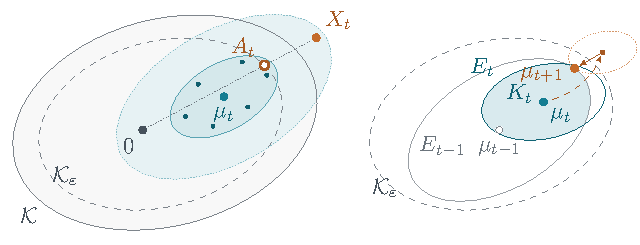
\includegraphics{figures/algorithm.pdf}
%     \caption{One round of \cref{alg:main}.
%         Left: the sample $X_t$ may fall outside $\K_\eps$, or even outside
%         $\K$. The learner plays the point $A_t$ where the segment from the
%         origin to $X_t$ meets the boundary of $\K_\eps$, and from its
%         observation computes a noisy value of $e_t(X_t)$.
%         Right: the focus region $K_t$ (shaded) is the intersection of
%         $\K_\eps$ with the ellipsoids of the epoch. When the Newton step
%         leaves $K_t$, the mean is projected back in the norm
%         $\normm{\cdot}{\Sigma_{t+1}^{-1}}$; the dotted ellipse is the ball of this
%         norm that touches $K_t$ at $\mu_{t+1}$. Here the active constraint
%     comes from the earlier ellipsoid $E_{t-1}$.}
%     \label{fig:algorithm}
% \end{figure}

\paragraph{The focus region and the restart test.}
The quadratic model is a faithful proxy for $e_t$ only near the current mean, so the algorithm keeps its mean in the \textit{focus region} $K_t=K_{t-1}\cap E_t$, where $K_0=\K_\eps$ and
\begin{align}
    E_t=\bigl\{x\in\R^d:\normm{x-\mu_t}{\Sigma_t^{-1}}^2\leq R^2\bigr\}.
\end{align}
The algorithm runs in epochs. Each epoch starts from $\mu_1=0$, $\Sigma_1=\sigma^2I_d$ and $K_0=\K_\eps$, with the round index starting again from one, and ends when the following test fires.
Let $Q_t=\sum_{s=1}^tq_s$. Since $q_s(\mu_s)=0$, the regret of the means $\mu_1,\ldots,\mu_t$ on $q_1,\ldots,q_t$ against a point $x$ is $-Q_t(x)$.
The test checks whether this regret is very negative against every point of $K_t$, that is, whether $\min_{x\in K_t}Q_t(x)$ is large.
Since $Q_t$ need not be convex, the algorithm works instead with
\begin{align}
    J_t(x)=\eta Q_t(x)+\normm{x}{\Sigma_1^{-1}}^2,
\end{align}
whose Hessian is $2\Sigma_{t+1}^{-1}\succ0$ by \cref{eq:updates}. It finds a point $y_t$ with
\begin{align}
    y_t\in K_t
    \qquad\text{and}\qquad
    J_t(y_t)\leq\min_{x\in K_t}J_t(x)+\frac\rho8,
    \eqlabel{eq:restart}
\end{align}
and restarts if $\eta Q_t(y_t)\geq2\rho$.
In \cref{pop:section} we show why an epoch that ends in a restart
has nonpositive regret against every point of $\K_\eps$.

% \paragraph{The focus region and the restart test.}
% Even the expected quadratic model $\bar{q}_t$ is a faithful proxy for $e_t$ only in an ellipsoid
% \begin{align}
%     E_t=\bigl\{x\in\R^d:\normm{x-\mu_t}{\Sigma_t^{-1}}^2\leq R^2\bigr\}
% \end{align}
% around the current mean $\mu_t$, where $R>0$ is a parameter of the algorithm.
% We define the \textit{focus region} in round $t$ by $K_t=K_{t-1}\cap E_t$ with $K_0=\K_\eps$.
% At the start, and again after every restart, $\mu_1=0$ and
% $\Sigma_1=\sigma^2I_d$, so $E_1$ is the ball of radius $R\sigma$ around the
% origin.
% As curvature accumulates in the
% inverse covariance, the ellipsoids narrow in the directions in which the losses are
% curved: $\Sigma_{t+1}^{-1}=\Sigma_t^{-1}+\frac{\eta\lambda}{2}H_t\succ \Sigma_t^{-1}$.

% The algorithm runs in epochs. An epoch ends when the restart test described
% below fires, and the next round starts a new epoch from the initial state
% $\mu_1=0$, $\Sigma_1=\sigma^2I_d$ and $K_0=\K_\eps$, with the round index $t$
% starting again from one and the losses relabelled in the same way.

% The test is about the regret of the means on the quadratic models. Within an
% epoch, let $Q_t=\sum_{s=1}^tq_s$ and $\bar{Q}_t=\sum_{s=1}^t\bar{q}_s$.
% Since we have $q_s(\mu_s)=0$, the regret of the means
% $\mu_1,\ldots,\mu_t$ against a competitor $x$ on the quadratic models is
% \begin{align}
%     \sum_{s=1}^t\bigl(q_s(\mu_s)-q_s(x)\bigr)=-Q_t(x).
%     \eqlabel{eq:Q_t-really}
% \end{align}
% An online learner usually wants this regret to be small.
% The restart test looks for the extreme case: it fires when the regret is
% not only small, but
% \emph{very negative} against every competitor $x\in K_t$ in the focus region.
% In terms of the cumulative model, by \cref{eq:Q_t-really},
% this happens when $\min_{x\in K_t}Q_t(x)$ is large.
% The analysis shows that this makes the regret of the epoch with respect to the
% extensions nonpositive against every comparator in $\K_\eps$, inside the focus
% region or not.

% The algorithm does not need to compute the best quadratic competitor in the focus region
% exactly; it is enough to find a
% point $y_t \in K_t$ that approximately minimizes a regularized and strongly convex version of $Q_t$.
% Since $H_s$ can be indefinite, $Q_t$ need not be convex.
% The regularized version adds the strongly convex term $\normm{x}{\Sigma_1^{-1}}^2$ to $\eta Q_t$ reaching
% \begin{align}
%     J_t(x)=\eta Q_t(x)+\normm{x}{\Sigma_1^{-1}}^2.
% \end{align}
% By \cref{eq:updates}, $\eta\lambda\sum_{s=1}^tH_s=2(\Sigma_{t+1}^{-1}-\Sigma_1^{-1})$, so the
% Hessian of $J_t$ is
% $\eta\lambda\sum_{s=1}^tH_s+2\Sigma_1^{-1}=2\Sigma_{t+1}^{-1}$, which is positive definite as long
% as the algorithm runs so $J_t$ is strongly convex.
% The algorithm approximately minimizes $J_t$ over the focus
% region up to an error of $\rho/8$, to achieve a point $y_t$ that satisfies
% \begin{align}
%     y_t\in K_t
%     \qquad\text{and}\qquad
%     J_t(y_t)\leq\min_{x\in K_t}J_t(x)+\frac\rho8,
%     \eqlabel{eq:restart}
% \end{align}
% and restarts if $\eta Q_t(y_t)\geq2\rho$.
% We will show that this negative quadratic regret implies negative extension regret against every point of $\K_\eps$ which makes the total regret of the epoch nonpositive.

\paragraph{Computation.}
We assume that the gauge $\pi$ of $\K$ can be evaluated, which is needed to
compute $A_t$ and $Y_t$. Besides this, each round solves two convex problems
over $K_t$: the projection in \cref{eq:updates} and the minimization in
\cref{eq:restart}. Both have strongly convex quadratic objectives, and $K_t$
is the intersection of $\K_\eps$ with at most $t$ ellipsoids, so both can be
solved in time polynomial in $d$ and $t$.\alireza{More computational notes?}

\begin{theorem}
    \label{thm:main}
    Let $\delta\in(0,1/2)$, let $A$ be a sufficiently large universal
    constant, and let $L=100\log(100nd/\delta)$. Set
    \begin{align}
        \sigma=\frac{1}{M\sqrt d\,L^2}
        \qquad\text{and}\qquad
        \eta=\frac{1}{A\sigma L^3}\sqrt{\frac dn},
        \eqlabel{eq:parameters-free}
    \end{align}
    and from these define
    \begin{align}
        \rho=A^3\Bigl(\frac d\sigma\Bigr)^2,
        \qquad
        \lambda=\frac{1}{L\sqrt{A\rho}},
        \qquad
        R^2=\frac{1}{32\lambda^2L},
        \qquad
        \eps=\frac{\rho}{\eta n}.
        \eqlabel{eq:parameters-derived}
    \end{align}
    If $\eps\leq1/2$, run \cref{alg:main} with these parameters.
    Otherwise play a fixed action in $\K$.
    With probability at least $1-\delta$,
    \begin{align}
        \Reg_n\leq\frac{3\rho}{\eta}=3A^4d^2ML^5\sqrt n .
        \ineqlabel{eq:main-regret}
    \end{align}
\end{theorem}
We prove \cref{thm:main} in \cref{transfer:section}, building on the analysis of a population version of the algorithm in \cref{pop:section}.

The bound in \cref{thm:main} depends on the position of $\K$ through
$M$. Since $\K$ is known, the learner can choose the affine preprocessing so
that $M$ is small, and this does not change the regret: the learner applies
the change of coordinates to its actions, and the losses remain convex and
bounded. In coordinates in which $\K/d$ is in L\"owner position, that is, its
minimum-volume enclosing ellipsoid is the unit ball, John's theorem gives
$\mathbb B_1\subseteq\K\subseteq\mathbb B_d$, and
$\E[\pi(U)]\leq C\sqrt{\log(ed)/d}$ for a universal constant $C\geq1$
\citep[Table~10.1(a)]{lattimore2026bandit}. Since also
$d^{-1/2}\leq C\sqrt{\log(ed)/d}$, the definition in \cref{eq:M} gives
$M\leq C\sqrt{\log(ed)/d}$, and \cref{thm:main} yields, with probability at
least $1-\delta$,
\begin{align}
    \Reg_n=O\!\left(d^{3/2}\sqrt{\log(ed)}\,L^5\sqrt n\right)
    =\widetilde O(d^{3/2}\sqrt n)
\end{align}
for every convex body $\K$.
\FloatBarrier

\section{The Population Algorithm}
\label{pop:section}
\suppressfloats[t]
In this section we analyze a hypothetical \textit{population algorithm} that has access to the population gradient $\bar g_t = \E_t[g_t]$ and Hessian $\bar H_t = \E_t[H_t]$ in each round $t$.
Of course, such an algorithm is not implementable, but it serves as a useful theoretical tool for understanding the behavior of the actual sampled algorithm.
Our goal is to show that the population algorithm satisfies the regret bound of \cref{thm:main} in expectation, instead of with high probability.
Because the population algorithm uses the exact gradient and Hessian, there is no estimation error to control. This makes the analysis simpler, and it shows the main reason the sampled algorithm works without the extra work of concentration inequalities.\tor{But note that the magnitude of the estimators makes this a slightly unreliable way of estimating regret.}

Precisely, the population algorithm is \cref{alg:main} with $g_t$ and $H_t$ replaced by $\bar g_t$ and $\bar H_t$, and with this change carried through every quantity built from them.
For instance, the restart test \cref{eq:restart} uses $\bar Q_t=\sum_{s=1}^t\bar q_s$ in place of $Q_t$.
Throughout this section the index $t$ starts at one in each epoch, except in statements explicitly summed over all $n$ rounds.

\begin{proposition}[Population regret]\label{pop:oracle}
    Suppose the parameters are as in \cref{thm:main} and $\eps\leq 1/2$. Then, for the population algorithm and for any sequence of losses $(f_t)_{t=1}^n$, it holds that
    \begin{align}
        \eReg_n \triangleq
        \sup_{y\in\K_\eps}\sum_{t=1}^n\bigl(\E_t[e_t(X_t)]-e_t(y)\bigr)\leq \frac{\rho}{\eta}\,.
    \end{align}
\end{proposition}
We call $\eReg_n$ the \textit{extension regret}. It differs from the regret $\Reg_n$ in two ways: it evaluates the extensions $e_t$ at $X_t$ instead of $f_t$ at $A_t$, and it compares against points of $\K_\eps$ instead of $\K$.
\kevin{This whole argument about how we can just focus on $e_t$ instead of $f_t$ should be all the way at the top where you say the first hing we do is ``forget'' $f_t$ I put a note}
Still, a\tor{high probability?} bound on $\eReg_n$ gives a bound on $\E[\Reg_n]$. Indeed, $f_t(A_t)\leq e_t(X_t)$, and for every $x\in\K$ the point $(1-\eps)x$ lies in $\K_\eps$, where $e_t=f_t$ and convexity gives $f_t((1-\eps)x)\leq f_t(x)+\eps$.
Hence, $\E[\Reg_n] \leq \E[\eReg_n]+n\eps$.
Since each $e_t$ is Lipschitz and $\K_\eps$ is compact, the supremum in $\eReg_n$ is attained. We fix
\begin{align}
    x_\star\in\argmin_{u\in\K_\eps}\sum_{t=1}^n e_t(u),
\end{align}
so that $\eReg_n=\sum_{t=1}^n\bigl(\E_t[e_t(X_t)]-e_t(x_\star)\bigr)$. This is a single comparator for all $n$ rounds, used across restarts.\kevin{This whole argument about how we can just focus on $e_t$ instead of $f_t$ should be all the way at the top where you say the first hing we do is ``forget'' $f_t$ I put a note}

\paragraph{Step 1: We relate extension regret to quadratic regret.}
Looking closely at the population algorithm, the only information about the losses that it keeps is $\bar g_t$ and $\bar H_t$, and together these define the quadratic $\bar q_t$. Its updates and its restart test depend on the losses only through $\bar q_1,\ldots,\bar q_t$.
So the losses pass through three stages: the adversary chooses $f_t$, the algorithm extends it to $e_t$, and $e_t$ is then replaced by its quadratic approximation $\bar q_t$ at $\mu_t$.
The algorithm knows $\bar q_t$ completely, and on these quadratics it runs a variant of continuous exponential weights, just as in online learning with full information. \tor{or Online Newton step}
A natural first step is therefore to relate the extension regret $\eReg_n$, which we saw controls the actual regret, to the (full-information) regret on the quadratics.
Within an epoch, the \textit{quadratic regret} of the means against a point
$y\in\R^d$ is \tor{$\bar{\qReg}$ doesn't look very nice.}
\begin{align}
    \bar{\qReg}_t(y)
    \triangleq\sum_{s=1}^t\bigl(\bar q_s(\mu_s)-\bar q_s(y)\bigr)
    =-\bar Q_t(y),
    \eqlabel{pop:qreg}
\end{align}
where the equality uses $\bar q_s(\mu_s)=0$.
The link between the two regrets is the following lemma, proved in \cref{sw:section}.
\begin{restatable}[Regret switching]{lemma}{regretswitching}
    \label{sw:tangent}
    Suppose that $\eps\leq1/2$, $0\prec\Sigma_t\preceq4\sigma^2 I_d$ and $\mu_t\in\K_\eps$. With the parameters of \cref{thm:main}, for every $x_0\in E_t$ and every $x_\star\in\K_\eps$,
    \begin{align}
        F_{t,\Sigma_t}(\mu_t)-e_t(x_\star)
        \leq \bar q_t(\mu_t)-\bar q_t(x_\star)
        +\frac{\lambda}{2}\normm{x_0-x_\star}{\bar H_t}^2
        +2\tr(\bar H_t\Sigma_t)+n^{-3}.
    \end{align}
\end{restatable}
Let us pause to discuss this lemma. First, its hypotheses hold at every round of the population algorithm. We assume $\eps\leq1/2$. Each $\bar H_t$ is positive semidefinite, so the covariance only shrinks within an epoch and $\Sigma_t\preceq\Sigma_1=\sigma^2I_d$. Finally, $\mu_t\in\K_\eps$ because the mean update projects onto the focus region, which lies in $\K_\eps$.

The lemma bounds the extension regret of round $t$ against $x_\star$ by the quadratic regret against $x_\star$, plus three extra terms. The term $n^{-3}$ is negligible. After summing over rounds, the usual log-determinant argument controls the trace term. The remaining term, $\frac\lambda2\normm{x_0-x_\star}{\bar H_t}^2$, needs more care. The comparator $x_\star$ can be any point of $\K_\eps$, but $x_0$ has to lie in the current focus ellipsoid $E_t$, and we pay for the distance between $x_0$ and $x_\star$ in the norm given by $\bar H_t$. Since $x_0$ is free, the question is how to choose it, and we turn to this next.

\paragraph{Step 2: We choose $x_0$ in the focus region.}
Fix an epoch and a round $t$ in it, so that the restart test has not been triggered in rounds $1,\ldots,t-1$. Since $K_t\subseteq E_s$ for every $s\leq t$, a single point $x_0\in K_t$ can be used in \cref{sw:tangent} in every round $s\leq t$. Write
\begin{align}
    c_s=2\tr(\bar H_s\Sigma_s)+n^{-3}
\end{align}
for the trace term and the negligible term together. We show later the bound on $\sum_{s=1}^t c_s$.
Summing \cref{sw:tangent} over $s=1,\ldots,t$ gives
\begin{align}
    \sum_{s=1}^t\bigl(F_{s,\Sigma_s}(\mu_s)-e_s(x_\star)\bigr)
    \leq \bar{\qReg}_t(x_\star)
    +\frac{\lambda}{2}\sum_{s=1}^t\normm{x_0-x_\star}{\bar H_s}^2
    +\sum_{s=1}^t c_s.
\end{align}
Since $\bar Q_t$ is a quadratic with Hessian $\lambda\sum_{s=1}^t\bar H_s$, the middle term equals
\begin{align}
    \frac{\lambda}{2}\sum_{s=1}^t\normm{x_0-x_\star}{\bar H_s}^2
    =\bar Q_t(x_\star)-\bar Q_t(x_0)-\ip{\nabla\bar Q_t(x_0)}{x_\star-x_0}.
\end{align}
By \cref{pop:qreg}, $\bar{\qReg}_t(x_\star)=-\bar Q_t(x_\star)$, so the first two terms on the right combine to give
\begin{align}
    \sum_{s=1}^t\bigl(F_{s,\Sigma_s}(\mu_s)-e_s(x_\star)\bigr)
    \leq \bar{\qReg}_t(x_0)
    -\ip{\nabla\bar Q_t(x_0)}{x_\star-x_0}
    +\sum_{s=1}^t c_s.
    \ineqlabel{pop:switch-sum}
\end{align}
The quadratic regret against $x_\star$ has become the quadratic regret against $x_0$, a point in the focus region.
The algorithm controls this regret: it runs a variant of exponential weights on the quadratics $\bar q_s$, which it sees in full, and we bound this regret in Step~3. That leaves the inner product. Because $\bar Q_t$ is convex, whenever $x_0$ minimizes $\bar Q_t$ over $\K_\eps$ the inner product is nonnegative, so the term $-\ip{\nabla\bar Q_t(x_0)}{x_\star-x_0}$ can be dropped.

This suggests choosing $x_0$ as a minimizer of the cumulative quadratic. Since $x_0$ must lie in $K_t$, we take
\begin{align}
    x^q_t\in\argmin_{u\in K_t}\bar Q_t(u).
\end{align}
To see why this is a good choice, suppose for the moment that $x^q_t$ also minimizes $\bar Q_t$ over all of $\K_\eps$, then the inner product term can be dropped, and the extension regret over rounds $1,\ldots,t$ is at most $\bar{\qReg}_t(x^q_t)+\sum_{s=1}^tc_s$, and both terms are under control.
Later, we will show that it does minimize $\bar Q_t$ over $\K_\eps$ as long as the epoch continues.

\paragraph{Step 3: We bound the quadratic regret of the online Newton step.}
We now bound the quadratic regret $\bar{\qReg}_t(x_0)$ against points $x_0\in K_t$.\alireza{say something about what ONS is.}
The Hessian of $\bar q_t$ is $\lambda\bar H_t$, but the update of the inverse covariance adds only $\eta\lambda\bar H_t/2$. As a result, the usual bound for the online Newton step comes with an extra negative term which will be useful later.
\begin{lemma}\label{pop:ons-lemma}
    For every $x_0\in K_t$, the population algorithm satisfies
    \begin{align}
        \bar{\qReg}_t(x_0)
        \leq \frac{\normm{\mu_1 - x_0}{\Sigma_1^{-1}}^2
        -\normm{\mu_{t+1}-x_0}{\Sigma_{t+1}^{-1}}^2}{2\eta}
        +\frac{\eta}{2}\sum_{s=1}^t\normm{\bar g_s}{\Sigma_{s+1}}^2
        -\frac{\lambda}{4}\sum_{s=1}^t\normm{x_0-\mu_s}{\bar H_s}^2.
        \ineqlabel{pop:ons-bound}
    \end{align}
\end{lemma}
\begin{proof}
    Fix $s\leq t$. Since $K_t\subseteq K_s$, the point $x_0$ lies in $K_s$, and $\mu_{s+1}$ is the projection of $\mu_s-\eta\Sigma_{s+1}\bar g_s$ onto $K_s$ in the norm $\normm{\cdot}{\Sigma_{s+1}^{-1}}$. Hence
    \begin{align}
        \frac12\normm{\mu_{s+1}-x_0}{\Sigma_{s+1}^{-1}}^2
        &\explan{\leq}{a}\frac12\normm{\mu_s-\eta\Sigma_{s+1}\bar g_s-x_0}{\Sigma_{s+1}^{-1}}^2\nonumber\\
        &=\frac12\normm{\mu_s-x_0}{\Sigma_{s+1}^{-1}}^2
        -\eta\ip{\bar g_s}{\mu_s-x_0}
        +\frac{\eta^2}{2}\normm{\bar g_s}{\Sigma_{s+1}}^2\nonumber\\
        &\explan{=}{b}\frac12\normm{\mu_s-x_0}{\Sigma_s^{-1}}^2
        +\frac{\eta\lambda}{4}\normm{x_0-\mu_s}{\bar H_s}^2
        -\eta\ip{\bar g_s}{\mu_s-x_0}
        +\frac{\eta^2}{2}\normm{\bar g_s}{\Sigma_{s+1}}^2\nonumber\\
        &\explan{=}{c}\frac12\normm{\mu_s-x_0}{\Sigma_s^{-1}}^2
        -\eta\bigl(\bar q_s(\mu_s)-\bar q_s(x_0)\bigr)
        -\frac{\eta\lambda}{4}\normm{x_0-\mu_s}{\bar H_s}^2
        +\frac{\eta^2}{2}\normm{\bar g_s}{\Sigma_{s+1}}^2.
    \end{align}
    Here \reason{a} holds because projecting onto the convex set $K_s$ does not increase the distance to $x_0\in K_s$, \reason{b} uses $\Sigma_{s+1}^{-1}-\Sigma_s^{-1}=\eta\lambda\bar H_s/2$, and \reason{c} uses \cref{eq:quadratic-model} and $\bar q_s(\mu_s)=0$. Summing over $s=1,\ldots,t$ telescopes the distance terms, and rearranging with $\mu_1=0$ gives the claim.
\end{proof}

We now combine the two lemmas. Taking $x_0=x^q_t\in K_t$ in \cref{pop:switch-sum} and bounding $\bar{\qReg}_t(x^q_t)$ by \cref{pop:ons-lemma} gives
\begin{align}
    \sum_{s=1}^t\bigl(F_{s,\Sigma_s}(\mu_s)-e_s(x_\star)\bigr)
    &\leq \frac{\normm{x^q_t}{\Sigma_1^{-1}}^2
    -\normm{\mu_{t+1}-x^q_t}{\Sigma_{t+1}^{-1}}^2}{2\eta}
    +\frac{\eta}{2}\sum_{s=1}^t\normm{\bar g_s}{\Sigma_{s+1}}^2
    +\sum_{s=1}^tc_s\nonumber\\
    &\quad-\frac{\lambda}{4}\sum_{s=1}^t\normm{x^q_t-\mu_s}{\bar H_s}^2
    -\ip{\nabla\bar Q_t(x^q_t)}{x_\star-x^q_t}.
    \ineqlabel{pop:combined}
\end{align}
The first line contains the terms of the usual bound for the online Newton step, together with $\sum_{s=1}^tc_s$. The two terms on the second line are new.
The first is nonpositive term we got from \cref{pop:ons-lemma} and the second is nonpositive whenever $x^q_t$ minimizes $\bar Q_t$ over $\K_\eps$ as we discussed earlier\alireza{in step..}.

\paragraph{Step 4: $x^q_t$ is a global minimizer.}
Suppose first that $x^q_t$ minimizes $\bar Q_t$ over all of $\K_\eps$. Then the inner product in \cref{pop:combined} is nonnegative, so the last term there is nonpositive. We drop it, along with the other two nonpositive terms.
By $c_s=2\tr(\bar H_s\Sigma_s)+n^{-3}$ we have
\begin{align}
    \sum_{s=1}^t\bigl(F_{s,\Sigma_s}(\mu_s)-e_s(x_\star)\bigr)
    \leq \frac{\normm{x^q_t}{\Sigma_1^{-1}}^2}{2\eta}
    +\frac{\eta}{2}\sum_{s=1}^t\normm{\bar g_s}{\Sigma_{s+1}}^2
    +2\sum_{s=1}^t\tr(\bar H_s\Sigma_s)
    +tn^{-3}.
    \ineqlabel{pop:easy}
\end{align}
The first term is at most $2d^2/(\eta\sigma^2)$, since $\Sigma_1=\sigma^2I_d$ and $\|x^q_t\|\leq2d$ because $\K_\eps\subseteq\K\subseteq\mathbb B_{2d}$. The other two sums are controlled by the following lemma, which we prove in \cref{pop:appendix}.
\begin{lemma}\label{pop:sums}
    For every epoch of the population algorithm and every round $t$ in it,
    \begin{align}
        \sum_{s=1}^t\tr(\bar H_s\Sigma_s)\leq\frac{16dL}{\lambda\eta}
        \qquad\text{and}\qquad
        \sum_{s=1}^t\normm{\bar g_s}{\Sigma_{s+1}}^2\leq5n.
    \end{align}
\end{lemma}
\alireza{double check the constants in the lemma.}
Substituting these bounds into \cref{pop:easy} and using $t\leq n$, we get, whenever $x^q_t$ minimizes $\bar Q_t$ over $\K_\eps$,
\begin{align}
    \sum_{s=1}^t\bigl(F_{s,\Sigma_s}(\mu_s)-e_s(x_\star)\bigr)
    \leq \frac{2d^2}{\eta\sigma^2}+\frac{5\eta n}{2}+\frac{32dL}{\lambda\eta}+n^{-2}
    \leq\frac{\rho}{\eta},
\end{align}
where the last inequality uses \cref{eq:parameters-free,eq:parameters-derived}.

This is the bound of \cref{pop:oracle}, but only under the assumption that $x^q_t$ minimizes $\bar Q_t$ over $\K_\eps$.
If $x^q_t$ does not minimize $\bar Q_t$ over $\K_\eps$, then it lies on the boundary of some focus ellipsoid $E_r$ with $r\leq t$.
Indeed, otherwise $x^q_t$ lies in the interior of each of $E_1,\ldots,E_t$, so $K_t$ and $\K_\eps$ coincide near $x^q_t$. Then $x^q_t$ is a local minimizer of $\bar Q_t$ over $\K_\eps$, and since $\bar Q_t$ is convex, it minimizes $\bar Q_t$ over $\K_\eps$.
We turn to this case next.

\paragraph{Step 5: Touching a focus ellipsoid forces a restart.}
We now prove that if $x^q_t$ lies on the boundary of an earlier focus ellipsoid $E_r$, then the restart test fires at round $t$.
In a later step we show that an epoch that ends in a restart has nonpositive extension regret.
Together with Step 4, this covers every epoch.
It is worth mentioning that we do not need to show that every restart is triggered by $x^q_t$ touching a focus ellipsoid.
The algorithm may restart for other reasons, and the analysis still holds.

Concretely, suppose that $x^q_t$ lies on the boundary of $E_r$ for some $r\leq t$, then
we prove that $\bar{\qReg}_t(x^q_t) = -\bar Q_t(x^q_t)$ is too negative, so $\bar Q_t(y_t)\geq\bar Q_t(x^q_t)$ is too large, and the test fires.
First, the quadratic regret against $x^q_t \in \K_t$ is bounded by \cref{pop:ons-lemma} at $x_0=x^q_t$:
\begin{align}
    -\bar Q_t(x^q_t)=\bar{\qReg}_t(x^q_t)
    \leq \frac{\normm{x^q_t-\mu_1}{\Sigma_1^{-1}}^2}{2\eta}
    +\frac{\eta}{2}\sum_{s=1}^t\normm{\bar g_s}{\Sigma_{s+1}}^2
    -\frac{\lambda}{4}\sum_{s<r}\normm{x^q_t-\mu_s}{\bar H_s}^2,
    \label{eq:pop-quad-reg}
\end{align}
where we deliberately dropped the nonnegative terms in the last sum over $s \in [r,t]$.
On the other hand, from $x^q_t \in \partial E_r$ we get
\begin{align}
    R^2
    = \normm{x^q_t - \mu_r}{\Sigma_r^{-1}}^2
    = \normm{x^q_t - \mu_r}{\Sigma_1^{-1}}^2
    + \frac{\eta\lambda}{2}\sum_{s<r}\normm{x^q_t - \mu_r}{\bar H_s}^2.
    \label{eq:pop-ellipsoid-boundary}
\end{align}
By adding and subtracting \cref{eq:pop-ellipsoid-boundary} divided by $2\eta$ to the RHS of \cref{eq:pop-quad-reg}, we get
\begin{align}
    \bar{\qReg}_t(x^q_t)
    &\leq
    -\frac{R^2}{2\eta}
    + \frac{
        \normm{x^q_t-\mu_1}{\Sigma_1^{-1}}^2 +
        \normm{x^q_t-\mu_r}{\Sigma_1^{-1}}^2
    }{2\eta}
    +\frac{\eta}{2}\sum_{s=1}^t\normm{\bar g_s}{\Sigma_{s+1}}^2
    \\
    &\quad+\frac{\lambda}{4}\sum_{s<r}\left( \normm{x^q_t-\mu_r}{\bar H_s}^2 - \normm{x^q_t-\mu_s}{\bar H_s}^2 \right) \\
    &\leq
    -\frac{R^2}{2\eta}
    +
    \frac{(4d)^2}{\eta\sigma^2}
    + \frac{5\eta n}{2}
    +\frac{\lambda}{4}\sum_{s<r}
    \Bigl(\frac12\normm{x^q_t-\mu_r}{\bar H_s}^2+\normm{\mu_r-\mu_s}{\bar H_s}^2\Bigr)\\
    &\leq-\frac{R^2}{4\eta}
    +\frac{(4d)^2}{\eta\sigma^2}
    +\frac{5\eta n}{2}
    +\frac{\lambda}{4}\sum_{s<r}\normm{\mu_s-\mu_r}{\bar H_s}^2,
    \ineqlabel{pop:boundary-movement}
\end{align}
where the second inequality uses \cref{pop:sums} together with $x^q_t, \mu_1, \mu_r \in \K_\eps \subseteq \K \subseteq \mathbb B_{2d}$,
and the inequality $\normm{x^q_t-\mu_s}{\bar H_s}^2 + \normm{\mu_r-\mu_s}{\bar H_s}^2 \geq \frac12\normm{x^q_t-\mu_r}{\bar H_s}^2$;
the last inequality uses \cref{eq:pop-ellipsoid-boundary} which shows that $\frac{\lambda}{8}\sum_{s<r}\normm{x^q_t-\mu_r}{\bar H_s}^2\leq\frac{R^2}{4\eta}$.
It remains to bound the last sum, which essentially measures how far the means $\mu_s$ have moved before round $r$.
The means cannot have moved far before round $r$, because the restart test did not fire at round $r-1$. A short calculation in \cref{pop:appendix}, which applies \cref{pop:ons-lemma} at round $r-1$, makes this precise:
\begin{align}
    \frac{\lambda}{4}\sum_{s<r}\normm{\mu_s-\mu_r}{\bar H_s}^2
    \leq\frac{1}{\eta}\Bigl(\frac{4d^2}{\sigma^2}+4\rho\Bigr)+5\eta n.
    \ineqlabel{pop:movement}
\end{align}
Substituting this into \cref{pop:boundary-movement} and multiplying by $\eta$,
\begin{align}
    \eta\,\bar{\qReg}_t(x^q_t)
    \leq-\frac{R^2}{4}+\frac{20d^2}{\sigma^2}+4\rho+\frac{15\eta^2n}{2}
    \leq-2\rho,
\end{align}
where the last inequality uses $d^2/\sigma^2=\rho/A^3$, $\eta^2n=\rho/(A^5dL^6)$ and $R^2\geq256\rho$. Finally, $y_t\in K_t$ and $x^q_t$ minimizes $\bar Q_t$ over $K_t$, so
\begin{align}
    \eta\bar Q_t(y_t)\geq\eta\bar Q_t(x^q_t)=-\eta\,\bar{\qReg}_t(x^q_t)\geq2\rho,
\end{align}
and the restart test fires at round $t$.
Consequently, if the restart test does not fire in rounds $1,\ldots,t$, then $x^q_t$ lies on none of the boundaries of $E_1,\ldots,E_t$, and so, by the end of Step 4, it minimizes $\bar Q_t$ over $\K_\eps$.

\paragraph{Step 6: $x^q_t$ stays in the focus region.}
We now prove that if round $t$ does not restart, then $x^q_t\in K_{t+1}$. We use this fact in the next step.
Since $x^q_t\in K_t$, it suffices to show $x^q_t\in E_{t+1}$. The test did not fire and $y_t\in K_t$, so $\eta\bar Q_t(x^q_t)\leq\eta\bar Q_t(y_t)<2\rho$. Applying \cref{pop:ons-lemma} with $x_0=x^q_t$, using $\bar{\qReg}_t(x^q_t)=-\bar Q_t(x^q_t)$, and dropping the curvature term gives
\begin{align}
    \frac12\normm{\mu_{t+1}-x^q_t}{\Sigma_{t+1}^{-1}}^2
    \leq\frac12\normm{x^q_t}{\Sigma_1^{-1}}^2
    +\frac{\eta^2}{2}\sum_{s=1}^t\normm{\bar g_s}{\Sigma_{s+1}}^2
    +\eta\bar Q_t(x^q_t)
    \leq\frac{2d^2}{\sigma^2}+\frac{5\eta^2n}{2}+2\rho
    \leq\frac{5\rho}{2},
\end{align}
where we used $\|x^q_t\|\leq2d$, \cref{pop:sums}, and $2d^2/\sigma^2+5\eta^2n/2\leq\rho/2$, which follows from \cref{eq:parameters-free,eq:parameters-derived}. Hence $\normm{\mu_{t+1}-x^q_t}{\Sigma_{t+1}^{-1}}^2\leq5\rho<R^2$, that is, $x^q_t\in E_{t+1}$.

\paragraph{Step 7: An epoch that ends in a restart has nonpositive regret.}
Suppose round $t$ ends the epoch in a restart, and let $z=x^q_{t-1}$, with $z=0$ if $t=1$. Rounds $1,\ldots,t-1$ did not restart, so by Step 5 the point $z$ minimizes $\bar Q_{t-1}$ over $\K_\eps$, and by Step 6 $z \in K_t$.

% We use $z$ as the comparator in place of $x_\star$.
For the first $t-1$ rounds, apply \cref{pop:switch-sum} at round $t-1$ with $x_0=z$. The inner product there is nonnegative because $z$ minimizes $\bar Q_{t-1}$ over $\K_\eps$, so
\begin{align}
    \sum_{s=1}^{t-1}\bigl(F_{s,\Sigma_s}(\mu_s)-e_s(x_\star)\bigr)
    \leq \bar{\qReg}_{t-1}(z)+\sum_{s=1}^{t-1}c_s.
    \ineqlabel{pop:first-rounds}
\end{align}
For the last round, apply \cref{sw:tangent} with both points equal to $z$, which removes the quadratic term. Since $e_t$ takes values in $[0,1]$ on $\K_\eps$, we have
\begin{align}
    F_{t,\Sigma_t}(\mu_t)-e_t(x_\star)
    =F_{t,\Sigma_t}(\mu_t)-e_t(z)+e_t(z)-e_t(x_\star)
    \leq \bar q_t(\mu_t)-\bar q_t(z)+c_t+1.
    \ineqlabel{pop:last-round}
\end{align}
Adding the two bounds, and using $\bar{\qReg}_t(z)=-\bar Q_t(z)$, gives
\begin{align}
    \sum_{s=1}^{t}\bigl(F_{s,\Sigma_s}(\mu_s)-e_s(x_\star)\bigr)
    \leq -\bar Q_t(z)+\sum_{s=1}^{t}c_s+1.
    \ineqlabel{pop:restart-sum}
\end{align}
It remains to show that $\bar Q_t(z)$ is large, and the restart test gives exactly this. Since $z\in K_t$, the definition of $y_t$ in \cref{eq:restart} gives $J_t(y_t)\leq J_t(z)+\rho/8$, that is,
\begin{align}
    \eta\bar Q_t(z)
    \geq\eta\bar Q_t(y_t)+\normm{y_t}{\Sigma_1^{-1}}^2-\normm{z}{\Sigma_1^{-1}}^2-\frac{\rho}{8}
    \geq2\rho-\frac{4d^2}{\sigma^2}-\frac{\rho}{8}
    \geq\frac{7\rho}{4},
\end{align}
where the second inequality uses the restart condition $\eta\bar Q_t(y_t)\geq2\rho$ and $\|z\|\leq2d$, and the last uses $4d^2/\sigma^2\leq\rho/8$. By \cref{pop:sums} and \cref{eq:parameters-free,eq:parameters-derived}, $\eta\bigl(1+\sum_{s=1}^tc_s\bigr)\leq2\eta+32dL/\lambda\leq\rho/4$. Substituting both bounds into \cref{pop:restart-sum} gives
\begin{align}
    \eta\sum_{s=1}^{t}\bigl(F_{s,\Sigma_s}(\mu_s)-e_s(x_\star)\bigr)
    \leq-\frac{7\rho}{4}+\frac{\rho}{4}
    =-\frac{3\rho}{2}<0.
\end{align}
So every epoch that ends in a restart has negative extension regret against $x_\star$.

\paragraph{Step 8: We sum over epochs.}
We now return to calendar time and prove \cref{pop:oracle}. The $n$ rounds split into epochs. By Step 7, every epoch that ends in a restart has negative extension regret against $x_\star$. If the last epoch does not end in a restart, let $t$ be its number of rounds. The restart test did not fire in any of these rounds, so by Step 5 the point $x^q_t$ minimizes $\bar Q_t$ over $\K_\eps$, and Step 4 bounds the extension regret of this epoch by $\rho/\eta$. If the last round ends in a restart, there is no such epoch. The comparator $x_\star$ is the same in every epoch, and $\E_t[e_t(X_t)]=F_{t,\Sigma_t}(\mu_t)$, so adding these bounds gives
\begin{align}
    \eReg_n=\sum_{t=1}^n\bigl(F_{t,\Sigma_t}(\mu_t)-e_t(x_\star)\bigr)\leq\frac{\rho}{\eta},
\end{align}
which proves \cref{pop:oracle}.

\section{Discussion}
\label{sec:discussion}
We gave an algorithm for adversarial bandit convex optimization with regret $\widetilde O(d^{3/2}\sqrt n)$ with high probability. It runs an online Newton step on quadratic models of the Gaussian smoothing of the loss, built from unbiased estimates of its gradient and Hessian. Its mean is kept inside a focus region, and it restarts when the restart test fires. The covariance update adds only half of the estimated curvature. The other half leaves a negative term, and the restart test uses this term to certify that an epoch has nonpositive regret.\tor{I never bother with these summaries. I don't believe anyone skips the introduction to read the discussion. Better just to focus on interesting things}

Several questions remain open. The bound matches the rate conjectured by \citet{bubeck2017kernel}. However, the lower bound of \citet{rajaraman2026price} is $\Omega(d^{4/3}\sqrt n)$, so the minimax regret is known only up to a factor of $d^{1/6}$. Our bound also carries the factor $L^5$, and we do not know how far the logarithmic factors can be reduced. Finally, within an epoch the focus region is an intersection of up to $t$ ellipsoids, so the computation per round grows polynomially with $n$. \citet[Conjecture~1]{bubeck2017kernel} asks for regret $\widetilde O(d^{3/2}\sqrt n)$ with computation per round polynomial in $d$ and $\log n$. It would be interesting to know whether the algorithm can keep only a bounded number of ellipsoids without losing the rate.\tor{bounded by what? It's hard to believe an absolute constant will be enough, but logarithmic is probably possible. Note, there is also the cost of the rounding. The L\"owner position is expensive. I believe that positioning $K$ so that it's polar is isotropic will also work and can be done in polynomial time.}

\newpage
\begingroup
\raggedright
\providecommand{\doi}[1]{\href{https://doi.org/#1}{doi:\nolinkurl{#1}}}
\bibliography{references}
\endgroup

\newpage
\appendix
\crefalias{section}{appendix}

\section{Omitted proofs from the population argument}\label{pop:appendix}

\begin{proof}[Proof of \cref{pop:sums}]
    The hypothesis \cref{fb:comparison} of \cref{fb:trace,fb:budget} holds with equality for the population algorithm. The first bound is therefore \cref{fb:trace-sum}.

    For the second bound, fix $s\leq t$ and let $Z_s=\Sigma_s^{-1/2}(X_s-\mu_s)$, which is standard Gaussian given the past. Since $\E_s[Y_s\mid X_s]=e_s(X_s)$, \cref{eq:gaussian-derivatives-estimates} gives $\Sigma_s^{1/2}\bar g_s=\E_s[e_s(X_s)Z_s]$. The coordinates of $Z_s$ are orthonormal in $L^2$, and the $i$th coordinate of $\E_s[e_s(X_s)Z_s]$ is the inner product of $e_s(X_s)$ with the $i$th coordinate of $Z_s$. So Bessel's inequality gives
    \begin{align}
        \normm{\bar g_s}{\Sigma_s}^2=\bigl\|\E_s[e_s(X_s)Z_s]\bigr\|^2\leq\E_s\bigl[e_s(X_s)^2\bigr].
    \end{align}
    Since $\bar H_s\succeq0$, we have $\Sigma_{s+1}\preceq\Sigma_s$, and hence $\normm{\bar g_s}{\Sigma_{s+1}}\leq\normm{\bar g_s}{\Sigma_s}$. Moreover, $\E_s[e_s(X_s)^2]\leq\E_s[Y_s^2]$, because $Y_s=e_s(X_s)+\pi_\eps(X_s)\xi_s$ and the noise has conditional mean zero. Summing over $s$ and applying \cref{fb:budget} proves the second bound.
\end{proof}

\begin{proof}[Proof of \cref{pop:movement}]
    Recall the setting of Step 5: the restart test has not fired in rounds $1,\ldots,t-1$, and $x^q_t$ lies on the boundary of $E_r$ for some $r\leq t$. If $r=1$, the sum is empty. Otherwise let $z=x^q_{r-1}$, and split each term at $z$:
    \begin{align}
        \frac{\lambda}{4}\sum_{s<r}\normm{\mu_s-\mu_r}{\bar H_s}^2
        &\leq\frac{\lambda}{2}\sum_{s<r}\normm{\mu_r-z}{\bar H_s}^2
        +\frac{\lambda}{2}\sum_{s<r}\normm{z-\mu_s}{\bar H_s}^2\\
        &\leq\frac{1}{\eta}\normm{\mu_r-z}{\Sigma_r^{-1}}^2
        +\frac{\lambda}{2}\sum_{s<r}\normm{z-\mu_s}{\bar H_s}^2,
    \end{align}
    where the second inequality uses $\frac{\eta\lambda}{2}\sum_{s<r}\bar H_s=\Sigma_r^{-1}-\Sigma_1^{-1}\preceq\Sigma_r^{-1}$. The right side is what the online Newton step controls at round $r-1$. Indeed, $z\in K_{r-1}$, and \cref{pop:ons-lemma} at round $r-1$ with $x_0=z$, multiplied by two and rearranged, gives
    \begin{align}
        \frac{1}{\eta}\normm{\mu_r-z}{\Sigma_r^{-1}}^2
        +\frac{\lambda}{2}\sum_{s<r}\normm{z-\mu_s}{\bar H_s}^2
        \leq\frac{\normm{z-\mu_1}{\Sigma_1^{-1}}^2}{\eta}
        +\eta\sum_{s<r}\normm{\bar g_s}{\Sigma_{s+1}}^2
        +2\bar Q_{r-1}(z).
    \end{align}
    The restart test did not fire at round $r-1$, and $z$ minimizes $\bar Q_{r-1}$ over $K_{r-1}$, which contains $y_{r-1}$. So $\eta\bar Q_{r-1}(z)\leq\eta\bar Q_{r-1}(y_{r-1})<2\rho$. Since $\mu_1=0$, $\|z\|\leq2d$ and $\Sigma_1=\sigma^2I_d$, the first term on the right is at most $4d^2/(\eta\sigma^2)$, and by \cref{pop:sums} the second is at most $5\eta n$. This proves the claim.
\end{proof}

\section{Properties of the convex extension}
\label{app:extension}

\begin{proof}[Proof of \cref{lem:extension}]
    Fix a loss $f$ and omit the round index. By
    \citet[Proposition~3.23]{lattimore2026bandit}, the function
    \begin{align}
        x\longmapsto
        \pi_\eps(x)f(x/\pi_\eps(x))+\frac{1-\eps}{\eps}v(x)
    \end{align}
    is convex. Since $v$ is convex, adding $v$ or $(1+\eps)v/\eps$ shows
    that $e-v/\eps$ and $e$ are convex, respectively.
    The equality on $\K_\eps$ and the inequality
    $f(x/\pi_\eps(x))\leq e(x)$ follow from the definition, since
    $\pi_\eps\geq1$, $v\geq0$ and $f\geq0$.

    To bound the Lipschitz constant, note that
    $0\leq e(x)\leq(1+2/\eps)\max\{1,\|x\|/(1-\eps)\}$ since $f\leq1$
    and $\pi(x)\leq\|x\|$. For $g\in\partial e(x)$ and a unit vector $u$,
    the subgradient inequality at $x+ru$ gives
    \begin{align}
        \ip{g}{u}\leq\limsup_{r\to\infty}\frac{e(x+ru)-e(x)}r
        \leq\frac{2+\eps}{\eps(1-\eps)}\leq\frac5\eps.
    \end{align}
    Taking a supremum over $u$ proves the claim.
\end{proof}

\section{Regret switching}
\label{sw:section}

\let\savedlabel\label\regretswitching*\global\let\label\savedlabel

The restriction on $x_0$ controls how far the slope of the quadratic
can depart from $\bar g_t$. The comparator $x_\star$ may be any point of
$\K_\eps$, including points outside the focus region.

\begin{proof}[Proof of \cref{sw:tangent}]
    \begingroup\allowdisplaybreaks[1]
    Fix the information available before the sample and suppress the round
    index. Write $e=e_t$, $X\sim\N(\mu,\Sigma)$ with $\mu=\mu_t$ and
    $\Sigma=\Sigma_t$, and
    \begin{align}
        F=F_{t,\Sigma_t}(\mu_t)=\E e(X),\qquad
        \bar g=\bar g_t,\qquad \bar H=\bar H_t,\qquad \bar q=\bar q_t.
    \end{align}
    All expectations in this proof are conditional on that information.
    In particular, $\bar q$ is the population quadratic, with Hessian
    $\lambda\bar H$, and $\bar q(\mu)=0$.
    We first give the calculation for a smooth convex $e$, so that
    $\bar g=\E\nabla e(X)$ and $\bar H=\E\nabla^2e(X)$. At the end we
    justify the same argument for the possibly nonsmooth extension.

    The exact quadratic expansion
    \begin{align}
        \bar q(x_\star)
        =\bar q(x_0)+\ip{\nabla\bar q(x_0)}{x_\star-x_0}
        +\frac\lambda2\normm{x_\star-x_0}{\bar H}^2
        \eqlabel{sw:derivation-tangent}
    \end{align}
    shows that our goal is to prove
    \begin{align}
        F-e(x_\star)
        &\leq \bar q(\mu)
        -\bigl(\bar q(x_0)+\ip{\nabla\bar q(x_0)}{x_\star-x_0}\bigr)
        +2\tr(\bar H\Sigma)+n^{-3}.
        \ineqlabel{sw:derivation-goal}
    \end{align}
    We will use two consequences of the parameters:
    \begin{align}
        \lambda&=\frac{1}{A^2d^{3/2}ML^3}\leq\frac{1}{8(d+L)},\qquad
        \lambda\normm{x_0-\mu}{\Sigma^{-1}}
        \leq\lambda R=\frac{1}{\sqrt{32L}}\leq\frac{1}{\sqrt{8L}}.
        \ineqlabel{sw:derivation-conditions}
    \end{align}
    The first follows from $M\geq d^{-1/2}$, $L\geq100$ and sufficiently
    large $A$; the second follows from $x_0\in E_t$ and the definition of $R$.

    For every sample $X$, the definition of the Bregman divergence gives
    \begin{align}
        e(X)-e(x_\star)
        =\ip{\nabla e(X)}{X-\mu}+\ip{\nabla e(X)}{\mu-x_\star}-D_e(x_\star\,\|\,X).
        \eqlabel{sw:derivation-starting-point}
    \end{align}
    Taking expectations,
    \begin{align}
        \E\bigl[e(X)-e(x_\star)\bigr]
        &=\E\bigl[\ip{\nabla e(X)}{X-x_\star}-D_e(x_\star\,\|\,X)\bigr]\\
        &=\E\ip{\nabla e(X)}{X-\mu}+\E\ip{\nabla e(X)}{\mu-x_\star}
        -\E\bigl[D_e(x_\star\,\|\,X)\bigr]\\
        &=\tr(\bar H\Sigma)+\ip{\nabla \bar q(\mu)}{\mu-x_\star}
        -\E\bigl[D_e(x_\star\,\|\,X)\bigr].
    \end{align}

    The goal is to make $\nabla \bar q(x_0)$ appear in place of $\nabla \bar q(\mu)$.
    Note that $\nabla \bar q(\mu)=\bar g$ came from the term $\E\nabla e(X)$.
    The key step is that there is a function
    \begin{align}
        w(x) = 1+\lambda\ip{x_0-\mu}{\Sigma^{-1}(x-\mu)}
    \end{align}
    such that
    \begin{align}
        \E[w(X) \nabla e(X)] = \nabla \bar q(x_0).
        \eqlabel{sw:derivation-key}
    \end{align}
    Indeed, Gaussian integration by parts gives
    $\E[\nabla e(X)(X-\mu)^\top]=\E[\nabla^2e(X)]\Sigma=\bar H\Sigma$, and therefore
    \begin{align}
        \E[w(X)\nabla e(X)]
        &=\E\nabla e(X)+\lambda\E\bigl[\nabla e(X)(X-\mu)^\top\bigr]\Sigma^{-1}(x_0-\mu)
        \nonumber\\
        &=\bar g+\lambda \bar H(x_0-\mu)
        =\nabla \bar q(x_0).
    \end{align}
    Moreover, $\E w(X)=1$. The weight can be negative, so it is not a
    probability density. Its connection with a change of Gaussian measure
    explains the choice of $w$.
    \paragraph{Where the weight comes from.}
    The weight is the first-order Taylor expansion of the Gaussian density
    ratio. More precisely, consider $\N(\mu+\lambda(x_0-\mu),\Sigma)$, the
    Gaussian moved a fraction $\lambda$ of the way from $\mu$ toward $x_0$.
    Its density with respect to $\N(\mu,\Sigma)$ is
    \begin{align}
        \frac{d\N(\mu+\lambda(x_0-\mu),\Sigma)}{d\N(\mu,\Sigma)}(x)
        &=\exp\Bigl(\lambda\ip{x_0-\mu}{\Sigma^{-1}(x-\mu)}
        -\frac{\lambda^2}{2}\normm{x_0-\mu}{\Sigma^{-1}}^2\Bigr)\nonumber\\
        &=1+\lambda\ip{x_0-\mu}{\Sigma^{-1}(x-\mu)}+O(\lambda^2)\nonumber\\
        &=w(x)+O(\lambda^2).
    \end{align}
    Here the expansion is for fixed $x$ as $\lambda\to0$. Thus $w$ is the
    linear approximation to the density ratio for this shift. The proof
    below uses the affine weight exactly, without a Taylor remainder.

    Now that we know how to get $\nabla \bar q(x_0)$, we can multiply \cref{sw:derivation-starting-point} by $w(X)$ and take expectations.
    The left-hand side becomes
    \begin{align}
        \E\bigl[w(X)\bigl(e(X)-e(x_\star)\bigr)\bigr]
        &\explan{=}{a}\E\bigl[w(X)e(X)\bigr]-e(x_\star)\nonumber\\
        &\explan{=}{b}F+\lambda\ip{x_0-\mu}{\Sigma^{-1}\E\bigl[(X-\mu)e(X)\bigr]}-e(x_\star)\nonumber\\
        &\explan{=}{c}F-e(x_\star)+\lambda\ip{x_0-\mu}{\bar g}.
        \eqlabel{sw:derivation-lhs}
    \end{align}
    Here \reason{a} uses $\E w(X)=1$; \reason{b} expands $w$ and uses $F=\E e(X)$; and
    \reason{c} uses Gaussian integration by parts,
    $\E[(X-\mu)e(X)]=\Sigma\,\E\nabla e(X)=\Sigma \bar g$.

    The right-hand side becomes
    \begin{align}
        &\E\Bigl[w(X)\Bigl(\ip{\nabla e(X)}{X-\mu}+\ip{\nabla e(X)}{\mu-x_\star}-D_e(x_\star\,\|\,X)\Bigr)\Bigr]\nonumber\\
        &\explan{=}{a}\E\bigl[w(X)\ip{\nabla e(X)}{X-\mu}\bigr]+\ip{\nabla \bar q(x_0)}{\mu-x_\star}
        -\E\bigl[w(X)D_e(x_\star\,\|\,X)\bigr]\nonumber\\
        &\explan{=}{b}\tr(\bar H\Sigma)+\lambda\ip{x_0-\mu}{\Sigma^{-1}\E\bigl[(X-\mu)\ip{\nabla e(X)}{X-\mu}\bigr]}\nonumber\\
        &\qquad+\ip{\nabla \bar q(x_0)}{\mu-x_\star}-\E\bigl[w(X)D_e(x_\star\,\|\,X)\bigr]\nonumber\\
        &\explan{=}{c}\tr(\bar H\Sigma)+\lambda\ip{x_0-\mu}{\E\bigl[\nabla^2e(X)(X-\mu)+\nabla e(X)\bigr]}\nonumber\\
        &\qquad+\ip{\nabla \bar q(x_0)}{\mu-x_\star}-\E\bigl[w(X)D_e(x_\star\,\|\,X)\bigr]\nonumber\\
        &\explan{=}{d}\tr(\bar H\Sigma)+\lambda\E\bigl[(x_0-\mu)^\top\nabla^2e(X)(X-\mu)\bigr]+\lambda\ip{x_0-\mu}{\bar g}\nonumber\\
        &\qquad+\ip{\nabla \bar q(x_0)}{\mu-x_\star}-\E\bigl[w(X)D_e(x_\star\,\|\,X)\bigr].
        \eqlabel{sw:derivation-rhs}
    \end{align}
    Here \reason{a} uses \cref{sw:derivation-key}; \reason{b} expands
    $w$ and uses $\E\ip{\nabla e(X)}{X-\mu}=\tr(\bar H\Sigma)$, which is Gaussian
    integration by parts; \reason{c} applies Gaussian integration by parts to
    $\varphi(X)=\ip{\nabla e(X)}{X-\mu}$, whose gradient is
    $\nabla^2e(X)(X-\mu)+\nabla e(X)$; and \reason{d} uses $\E\nabla e(X)=\bar g$.

    Now, note that the term $\lambda\ip{x_0-\mu}{\bar g}$ is present in both \cref{sw:derivation-lhs} and \cref{sw:derivation-rhs}, so we can cancel it out,
    and the weighted version of \cref{sw:derivation-starting-point} becomes
    \begin{align}
        F-e(x_\star)
        &=
        \tr(\bar H\Sigma)+\lambda\E\bigl[(x_0-\mu)^\top\nabla^2e(X)(X-\mu)\bigr]\nonumber\\
        &\qquad+\ip{\nabla \bar q(x_0)}{\mu-x_\star}-\E\bigl[w(X)D_e(x_\star\,\|\,X)\bigr].
        \eqlabel{sw:derivation-weighted}
    \end{align}
    Next we make the quadratic at $x_0$ appear. Since $\bar q$ is a quadratic with
    Hessian $\lambda \bar H$, its expansion around $x_0$ is exact,
    $\bar q(\mu)=\bar q(x_0)+\ip{\nabla \bar q(x_0)}{\mu-x_0}+\frac\lambda2\normm{\mu-x_0}{\bar H}^2$.
    Therefore
    \begin{align}
        F-e(x_\star)
        &\explan{=}{a}\tr(\bar H\Sigma)+\lambda\E\bigl[(x_0-\mu)^\top\nabla^2e(X)(X-\mu)\bigr]\nonumber\\
        &\qquad+\ip{\nabla \bar q(x_0)}{\mu-x_0}-\ip{\nabla \bar q(x_0)}{x_\star-x_0}-\E\bigl[w(X)D_e(x_\star\,\|\,X)\bigr]\nonumber\\
        &\explan{=}{b}\bar q(\mu)-\bigl(\bar q(x_0)+\ip{\nabla \bar q(x_0)}{x_\star-x_0}\bigr)+\tr(\bar H\Sigma)\nonumber\\
        &\qquad
        +\lambda\E\bigl[(x_0-\mu)^\top\nabla^2e(X)(X-\mu)\bigr]-\frac\lambda2\normm{x_0-\mu}{\bar H}^2
        \nonumber\\
        &\qquad-\E\bigl[w(X)D_e(x_\star\,\|\,X)\bigr].
        \eqlabel{sw:derivation-quadratic}
    \end{align}
    Here \reason{a} uses \cref{sw:derivation-weighted} and splits
    $\mu-x_\star=(\mu-x_0)-(x_\star-x_0)$; and \reason{b} uses the expansion of $\bar q$
    around $x_0$.
    The rest of the proof is to upper bound the last three terms in \cref{sw:derivation-quadratic}.

    \proofstepinline{1} We bound the curvature term.
    First we address the following term in \cref{sw:derivation-quadratic}:
    \begin{align}
        \lambda\E\bigl[(x_0-\mu)^\top\nabla^2e(X)(X-\mu)\bigr]-\frac\lambda2\normm{x_0-\mu}{\bar H}^2.
        \label{sw:derivation-step1}
    \end{align}
    First, we have
    \begin{align}
        &\E\bigl[(x_0-\mu)^\top\nabla^2e(X)(X-\mu)\bigr]\nonumber\\
        &\quad\explan{\le}{a}\frac12\E\bigl[(x_0-\mu)^\top\nabla^2e(X)(x_0-\mu)\bigr]
        +\frac12\E\bigl[(X-\mu)^\top\nabla^2e(X)(X-\mu)\bigr]\nonumber\\
        &\quad\explan{=}{b}\frac12\normm{x_0-\mu}{\bar H}^2+\frac12\E\normm{X-\mu}{\nabla^2e(X)}^2.
    \end{align}
    Here \reason{a} applies $2a^\top Ac\le a^\top Aa+c^\top Ac$, which holds for every
    $A\succeq0$ because $(a-c)^\top A(a-c)\ge0$, with $a=x_0-\mu$, $c=X-\mu$ and
    $A=\nabla^2e(X)\succeq0$ by convexity of $e$; and \reason{b} uses $\bar H=\E\nabla^2e(X)$.
    Consequently, considering the term in \cref{sw:derivation-step1}, we have
    \begin{align}
        \lambda\E\bigl[(x_0-\mu)^\top\nabla^2e(X)(X-\mu)\bigr]-\frac\lambda2\normm{x_0-\mu}{\bar H}^2
        \le\frac\lambda2\E\normm{X-\mu}{\nabla^2e(X)}^2.
        \ineqlabel{sw:derivation-step1-continued}
    \end{align}

    Now we bound the right-hand side of \cref{sw:derivation-step1-continued}.
    First, we standardize the sample. Let $Z=\Sigma^{-1/2}(X-\mu)\sim\mathcal N(0,I_d)$
    and $B=\Sigma^{1/2}\nabla^2e(X)\Sigma^{1/2}$, which is positive semidefinite by
    convexity of $e$. Then
    \begin{align}
        \normm{X-\mu}{\nabla^2e(X)}^2
        &\explan{=}{a}Z^\top BZ
        \explan{\le}{b}\|Z\|^2\tr(B)
        \explan{=}{c}\|Z\|^2\tr\bigl(\nabla^2e(X)\Sigma\bigr).
    \end{align}
    Here \reason{a} substitutes $X-\mu=\Sigma^{1/2}Z$; \reason{b} uses
    $z^\top Bz\le\|z\|^2\lambda_{\max}(B)\le\|z\|^2\tr(B)$, which holds for every
    $B\succeq0$; and \reason{c} uses the cyclic property of the trace.
    Taking expectations,
    \begin{align}
        \frac\lambda2\E\normm{X-\mu}{\nabla^2e(X)}^2
        \le\frac\lambda2\E\bigl[\|Z\|^2\tr\bigl(\nabla^2e(X)\Sigma\bigr)\bigr].
        \ineqlabel{sw:derivation-step1-1}
    \end{align}
    Compared with $\tr(\bar H\Sigma)=\E\tr(\nabla^2e(X)\Sigma)$, the only difference is
    the factor $\|Z\|^2$, which is about $d$ for a typical sample.

    Next we handle the typical samples. Let $r^2=16(d+L)$ and split the
    expectation in \cref{sw:derivation-step1-1} according to
    whether $\|Z\|^2\le r^2$. The part on this event satisfies
    \begin{align}
        \frac\lambda2\E\bigl[\|Z\|^2\tr\bigl(\nabla^2e(X)\Sigma\bigr)\1\{\|Z\|^2\le r^2\}\bigr]
        &\explan{\le}{a}\frac{\lambda r^2}2\E\bigl[\tr\bigl(\nabla^2e(X)\Sigma\bigr)\1\{\|Z\|^2\le r^2\}\bigr]\nonumber\\
        &\explan{\le}{b}\frac{\lambda r^2}2\E\tr\bigl(\nabla^2e(X)\Sigma\bigr)\nonumber\\
        &\explan{=}{c}8\lambda(d+L)\tr(\bar H\Sigma)\nonumber\\
        &\explan{\le}{d}\tr(\bar H\Sigma).
        \ineqlabel{sw:derivation-step1-2}
    \end{align}
    Here \reason{a} uses $\|Z\|^2\le r^2$ on the event; \reason{b} drops the indicator, which is
    allowed because $\tr(\nabla^2e(X)\Sigma)\ge0$; \reason{c} uses $\bar H=\E\nabla^2e(X)$ and
    $r^2=16(d+L)$; and \reason{d} uses $\lambda\le1/(8(d+L))$ from
    \cref{sw:derivation-conditions}.

    It remains to handle the atypical samples, $\|Z\|^2>r^2$. There the curvature
    of $e$ is not controlled by $\tr(\bar H\Sigma)$, so we use instead that these samples
    are exponentially rare and that $e$ is Lipschitz.
    Let $h(z)=e(\mu+\Sigma^{1/2}z)$, let $L_e$ be the Lipschitz constant of $e$, and
    let $s=\|\Sigma\|_{\op}^{1/2}$. Then $h$ is convex and $L_es$-Lipschitz, and
    $\Delta h(Z)=\tr(\nabla^2e(X)\Sigma)$, where $\Delta h\ge0$ by convexity. We write $\Delta h(dz)=\Delta h(z)\,dz$ in the integrals below.
    Write $\gamma_{0,I_d}$ and $\gamma_{0,2I_d}$ for the Gaussian densities with
    covariances $I_d$ and $2I_d$, and let $Z_2\sim\N(0,2I_d)$. Then
    \begin{align}
        &\frac\lambda2\E\bigl[\|Z\|^2\tr\bigl(\nabla^2e(X)\Sigma\bigr)\1\{\|Z\|^2>r^2\}\bigr]\nonumber\\
        &\quad\explan{=}{a}\frac\lambda2\int_{\|z\|^2>r^2}\|z\|^2\gamma_{0,I_d}(z)\,\Delta h(dz)\nonumber\\
        &\quad\explan{\le}{b}\frac\lambda2\,2^{d/2}e^{-r^2/4}\int\|z\|^2\gamma_{0,2I_d}(z)\,\Delta h(dz)\nonumber\\
        &\quad\explan{=}{c}-\frac\lambda2\,2^{d/2}e^{-r^2/4}\int\ip{\nabla h(z)}{\bigl(2-\|z\|^2/2\bigr)z}\gamma_{0,2I_d}(z)\,dz\nonumber\\
        &\quad\explan{\le}{d}\frac\lambda2\,2^{d/2}e^{-r^2/4}L_es\,\E\bigl[\bigl(2+\|Z_2\|^2/2\bigr)\|Z_2\|\bigr]\nonumber\\
        &\quad\explan{\le}{e}\frac\lambda2L_es\cdot5(d+2)^{3/2}2^{d/2}e^{-4(d+L)}\nonumber\\
        &\quad\explan{\le}{f}\frac\lambda2L_ese^{-4L}.
        \ineqlabel{sw:derivation-step1-3}
    \end{align}
    Here \reason{a} writes the expectation as an integral against the measure $\Delta h$;
    \reason{b} uses $\gamma_{0,I_d}(z)=2^{d/2}e^{-\|z\|^2/4}\gamma_{0,2I_d}(z)$ and
    $\|z\|^2>r^2$, and then enlarges the domain of a nonnegative integral;
    \reason{c} integrates by parts, using
    $\nabla\bigl(\|z\|^2\gamma_{0,2I_d}(z)\bigr)=(2-\|z\|^2/2)z\,\gamma_{0,2I_d}(z)$;
    \reason{d} uses the Cauchy--Schwarz inequality, $\|\nabla h\|\le L_es$ and
    $|2-\|z\|^2/2|\le2+\|z\|^2/2$;
    \reason{e} uses $\E\|Z_2\|\le\sqrt{2d}$ and
    $\E\|Z_2\|^3\le(\E\|Z_2\|^4)^{3/4}=(4d(d+2))^{3/4}$, which give
    $2\E\|Z_2\|+\frac12\E\|Z_2\|^3\le3\sqrt2(d+2)^{3/2}\le5(d+2)^{3/2}$,
    together with $r^2=16(d+L)$; and \reason{f} uses
    $5(d+2)^{3/2}2^{d/2}e^{-4d}\le1$ for every $d\ge1$, since the left-hand side
    is decreasing in $d$ and is less than one at $d=1$.

    Adding \cref{sw:derivation-step1-2,sw:derivation-step1-3}
    and using \cref{sw:derivation-step1-1}, we obtain
    \begin{align}
        \frac\lambda2\E\normm{X-\mu}{\nabla^2e(X)}^2\le\tr(\bar H\Sigma)+\frac\lambda2L_ese^{-4L}.
        \ineqlabel{sw:derivation-step1-final}
    \end{align}

    \proofstepinline{2} We control the negative part of the weight.
    Next we address the last term in \cref{sw:derivation-quadratic}:
    \begin{align}
        -\E\bigl[w(X)D_e(x_\star\,\|\,X)\bigr].
        \label{sw:derivation-step2}
    \end{align}
    Without the weight this term would be nonpositive, since
    $D_e(x_\star\,\|\,X)\ge0$ by convexity of $e$. With the weight it is still
    nonpositive on the event $w(X)\ge0$, but it can be positive on the event
    $w(X)<0$. We drop the first part and keep only the second:
    \begin{align}
        -\E\bigl[w(X)D_e(x_\star\,\|\,X)\bigr]
        &\explan{\le}{a}-\E\bigl[w(X)D_e(x_\star\,\|\,X)\1\{w(X)<0\}\bigr]
        \nonumber\\
        &\explan{=}{b}\E\bigl[(-w(X))_+D_e(x_\star\,\|\,X)\bigr].
        \ineqlabel{sw:derivation-step2-sign}
    \end{align}
    Here \reason{a} drops $-\E[w(X)D_e(x_\star\,\|\,X)\1\{w(X)\ge0\}]$, which is
    nonpositive; and \reason{b} uses $-w\1\{w<0\}=(-w)_+$.

    Convexity gives no upper bound on the Bregman divergence, so we use the
    Lipschitz constant of $e$ instead:
    \begin{align}
        D_e(x_\star\,\|\,X)
        &\explan{=}{a}e(x_\star)-e(X)-\ip{\nabla e(X)}{x_\star-X}\nonumber\\
        &\explan{\le}{b}2L_e\|x_\star-X\|\nonumber\\
        &\explan{\le}{c}2L_e\bigl(\|x_\star-\mu\|+\|\Sigma^{1/2}Z\|\bigr)\nonumber\\
        &\explan{\le}{d}2L_e\bigl(\|x_\star-\mu\|+s\|Z\|\bigr).
        \ineqlabel{sw:derivation-step2-bregman}
    \end{align}
    Here \reason{a} is the definition of the Bregman divergence; \reason{b} uses
    $|e(x_\star)-e(X)|\le L_e\|x_\star-X\|$, the Cauchy--Schwarz inequality and
    $\|\nabla e(X)\|\le L_e$; \reason{c} uses the triangle inequality and
    $X-\mu=\Sigma^{1/2}Z$; and \reason{d} uses $\|\Sigma^{1/2}\|_{\op}=s$.

    Next we write the weight in terms of $Z$. Let
    $a=\lambda\normm{x_0-\mu}{\Sigma^{-1}}$. If $a=0$, then $w=1$ and the
    right-hand side of \cref{sw:derivation-step2-sign} is
    zero, so assume $a>0$. Let
    $u=\Sigma^{-1/2}(x_0-\mu)/\normm{x_0-\mu}{\Sigma^{-1}}$, which is a unit
    vector, and write $Z=Gu+Z_\perp$ with $G=\ip uZ$. Then
    $G\sim\mathcal N(0,1)$ is independent of $Z_\perp$,
    $\|Z\|\le|G|+\|Z_\perp\|$, and
    $\E\|Z_\perp\|\le(\E\|Z_\perp\|^2)^{1/2}=\sqrt{d-1}\le\sqrt d$. Moreover,
    \begin{align}
        w(X)=1+\lambda\ip{\Sigma^{-1/2}(x_0-\mu)}{Z}=1+aG,
    \end{align}
    so $w(X)<0$ exactly when $G<-1/a$, and $(-w(X))_+=a(-G-1/a)_+$.
    We need two moments of $G$ on this event. Let $\phi$ and $\Phi$ be the
    standard Gaussian density and distribution function, and let $b>0$. Since
    $t\phi(t)=-\phi'(t)$, integration by parts gives
    \begin{align}
        \E\bigl[(-G-b)_+|G|\bigr]=\int_b^\infty(t-b)\,t\phi(t)\,dt=\Phi(-b),
    \end{align}
    and since $|G|\ge b$ wherever $(-G-b)_+>0$, also
    $\E(-G-b)_+\le\Phi(-b)/b$. Therefore
    \begin{align}
        &\E\bigl[(-w(X))_+D_e(x_\star\,\|\,X)\bigr]\nonumber\\
        &\quad\explan{\le}{a}2L_e\E\bigl[(-w(X))_+\bigl(\|x_\star-\mu\|+s\|Z\|\bigr)\bigr]\nonumber\\
        &\quad\explan{\le}{b}2L_ea\E\bigl[(-G-1/a)_+\bigl(\|x_\star-\mu\|+s\|Z_\perp\|+s|G|\bigr)\bigr]\nonumber\\
        &\quad\explan{=}{c}2L_ea\Bigl[\bigl(\|x_\star-\mu\|+s\E\|Z_\perp\|\bigr)\E(-G-1/a)_+
        +s\E\bigl[(-G-1/a)_+|G|\bigr]\Bigr]\nonumber\\
        &\quad\explan{\le}{d}2L_ea\Bigl[\bigl(\|x_\star-\mu\|+s\sqrt d\bigr)a\Phi(-1/a)+s\Phi(-1/a)\Bigr]\nonumber\\
        &\quad\explan{\le}{e}L_ea\bigl(a\|x_\star-\mu\|+s(1+a\sqrt d)\bigr)e^{-1/(2a^2)}\nonumber\\
        &\quad\explan{\le}{f}L_e\bigl(\|x_\star-\mu\|+2s\sqrt d\bigr)e^{-4L}.
        \ineqlabel{sw:derivation-step2-tail}
    \end{align}
    Here \reason{a} uses \cref{sw:derivation-step2-bregman};
    \reason{b} uses $(-w(X))_+=a(-G-1/a)_+$ and $\|Z\|\le|G|+\|Z_\perp\|$; \reason{c} uses
    the independence of $G$ and $Z_\perp$; \reason{d} uses $\E\|Z_\perp\|\le\sqrt d$
    and the two moments of $G$ with $b=1/a$; \reason{e} collects terms and uses
    $\Phi(-b)\le\frac12e^{-b^2/2}$; and \reason{f} uses $a\le1/\sqrt{8L}$ from
    \cref{sw:derivation-conditions}, which gives
    $e^{-1/(2a^2)}\le e^{-4L}$ and $a\le1$, together with $1\le\sqrt d$.

    Combining \cref{sw:derivation-step2-sign,sw:derivation-step2-tail}, we obtain
    \begin{align}
        -\E\bigl[w(X)D_e(x_\star\,\|\,X)\bigr]\le L_e\bigl(\|x_\star-\mu\|+2s\sqrt d\bigr)e^{-4L}.
        \ineqlabel{sw:derivation-step2-final}
    \end{align}

    \proofstepinline{3} We combine the bounds.
    Finally we put the two steps together. Bounding the last three terms of
    \cref{sw:derivation-quadratic} by
    \cref{sw:derivation-step1-continued,sw:derivation-step1-final,sw:derivation-step2-final}
    gives
    \begin{align}
        F-e(x_\star)
        &\le \bar q(\mu)-\bigl(\bar q(x_0)+\ip{\nabla \bar q(x_0)}{x_\star-x_0}\bigr)+2\tr(\bar H\Sigma)\nonumber\\
        &\qquad+\frac\lambda2L_ese^{-4L}+L_e\bigl(\|x_\star-\mu\|+2s\sqrt d\bigr)e^{-4L}.
        \ineqlabel{sw:derivation-step3-combined}
    \end{align}
    It remains to show that the last two terms are at most $n^{-3}$. We use four
    facts. First, $\lambda\le1$ by \cref{sw:derivation-conditions}.
    Second, $s\le1$: the covariance assumption in the lemma gives
    $\Sigma\preceq4\sigma^2I_d$, so
    $ s\le2\sigma=2/(M\sqrt d\,L^2)\le2/L^2\le1$, using
    $M\ge d^{-1/2}$ and $L\ge100$.
    Third, $\|x_\star-\mu\|\le4d$, since $x_\star\in\K_\eps$, the mean $\mu$ lies
    in $\K_\eps$ by assumption, and $\K_\eps\subseteq\K\subseteq\mathbb B_{2d}$.
    Fourth, $L_e\le5/\eps\le5\sqrt n$ by \cref{lem:extension}, since
    $\eps=A^4d^2ML^5/\sqrt n\ge1/\sqrt n$. Therefore
    \begin{align}
        \frac\lambda2L_ese^{-4L}+L_e\bigl(\|x_\star-\mu\|+2s\sqrt d\bigr)e^{-4L}
        &\explan{\le}{a}\Bigl(\frac12+4d+2\sqrt d\Bigr)L_ee^{-4L}\nonumber\\
        &\explan{\le}{b}7dL_ee^{-4L}\nonumber\\
        &\explan{\le}{c}35d\sqrt n\,e^{-4L}\nonumber\\
        &\explan{=}{d}35d\sqrt n\Bigl(\frac\delta{100nd}\Bigr)^{400}\nonumber\\
        &\explan{\le}{e}n^{-3}.
        \ineqlabel{sw:derivation-step3-error}
    \end{align}
    Here \reason{a} uses $\lambda\le1$, $s\le1$ and $\|x_\star-\mu\|\le4d$; \reason{b} uses
    $d\ge1$; \reason{c} uses $L_e\le5\sqrt n$; \reason{d} substitutes
    $L=100\log(100nd/\delta)$; and \reason{e} uses $\delta<1$ and $n,d\ge1$.
    Substituting \cref{sw:derivation-step3-error} into
    \cref{sw:derivation-step3-combined}, we obtain
    \begin{align}
        F-e(x_\star)
        \le \bar q(\mu)-\bigl(\bar q(x_0)+\ip{\nabla \bar q(x_0)}{x_\star-x_0}\bigr)+2\tr(\bar H\Sigma)+n^{-3}.
        \ineqlabel{sw:derivation-step3-final}
    \end{align}

    By \cref{sw:derivation-tangent}, this is precisely the stated inequality
    when $e$ is smooth.

    To remove the smoothness assumption, let
    $e_\tau(x)=\E_Z[e(x+\tau Z)]$ with $Z\sim\N(0,I_d)$ and $\tau>0$.
    Then $e_\tau$ is smooth and convex, has Lipschitz constant at most $L_e$,
    and satisfies
    \begin{align}
        \sup_{x\in\R^d}|e_\tau(x)-e(x)|\leq\tau L_e\E\|Z\|
        \longrightarrow0.
    \end{align}
    Apply the preceding calculation to $e_\tau$, defining $F_\tau$,
    $\bar g_\tau$, $\bar H_\tau$ and $\bar q_\tau$ by the same Gaussian
    averages and quadratic formula. All bounds use only the common
    Lipschitz bound, the covariance assumption and the displayed parameter
    conditions, so they hold uniformly in $\tau$. The Gaussian score
    identities in \cref{eq:gaussian-derivatives}, together with uniform
    convergence and integrability of the Gaussian scores, imply
    $F_\tau\to F$, $\bar g_\tau\to\bar g$ and
    $\bar H_\tau\to\bar H$. Hence $\bar q_\tau$ and its gradient converge
    at each fixed point. Passing to the limit gives
    \cref{sw:derivation-goal} for $e$, and
    \cref{sw:derivation-tangent} proves the lemma.
    \endgroup
\end{proof}

\section{Trace bound}
\label{app:trace}

The trace term in \cref{sw:tangent} measures the curvature of the
smoothed loss in the directions in which the sampling distribution is
wide. Indeed, the Jensen gap of the population quadratic is
\begin{align}
    \E_s[\bar q_s(X_s)]-\bar q_s(\mu_s)
    &=\frac\lambda2\E_s\bigl[(X_s-\mu_s)^\top\bar H_s(X_s-\mu_s)\bigr]
    =\frac\lambda2\tr(\bar H_s\Sigma_s).
\end{align}
The covariance update responds to this curvature. We will show that the
sum of the traces is controlled by a log-determinant ratio, and then
bound this ratio by controlling the growth of the inverse covariance.

Throughout this appendix, the parameters are those of \cref{thm:main},
with $\eps\leq1/2$. We will use their expanded form:
\begin{align}
    \sigma^2&=\frac{1}{dM^2L^4},&
    \eta&=\frac{dM}{AL\sqrt n},&
    \rho&=A^3d^3M^2L^4,\notag\\
    \lambda&=\frac{1}{A^2d^{3/2}ML^3},&
    \eps&=\frac{A^4d^2ML^5}{\sqrt n}.&&
    \eqlabel{eq:parameters}
\end{align}

Fix an epoch and number its rounds from one. Write
$W_s=X_s-\mu_s$ and $T_s=\tr(\bar H_s\Sigma_s)$, and define
\begin{align}
    \bar\Sigma_1=\Sigma_1=\sigma^2I_d,\qquad
    \bar\Sigma_{s+1}^{-1}
    =\bar\Sigma_s^{-1}+\frac{\lambda\eta}{2}\bar H_s.
    \eqlabel{fb:inverse-covariance}
\end{align}
Thus $\bar\Sigma_s^{-1}$ accumulates the conditional mean Hessians along
the sampled trajectory; note that $\bar\Sigma_s$ is not the expectation of
$\Sigma_s$.
Since $\bar H_s\succeq0$, the matrices
$\bar\Sigma_s^{-1}$ are nondecreasing and $\bar\Sigma_s\preceq\sigma^2I_d$.
The sampled Hessians can be indefinite, so we apply the log-determinant
argument to $\bar\Sigma_s$ and compare it with $\Sigma_s$.

We prove the bounds for every epoch prefix $0\leq t\leq n$ on which
\begin{align}
    \tfrac12\bar\Sigma_s^{-1}\preceq\Sigma_s^{-1}
    \preceq2\bar\Sigma_s^{-1}\qquad(1\leq s\leq t).
    \ineqlabel{fb:comparison}
\end{align}
This comparison is assumed only before the sample in each round.
In particular, the bounds include $\bar\Sigma_{t+1}$ even if the sampled
update at round $t$ is the first to violate \cref{fb:comparison}.
The concentration argument in \cref{conc:section} will establish that
this comparison holds throughout the algorithm with high probability.

\begin{lemma}[Growth of the inverse covariance]
    \label{fb:spectrum}
    Under \cref{fb:comparison},
    \begin{align}
        \|\bar\Sigma_{t+1}^{-1}\|_{\op}^{1/2}
        \leq\sigma^{-1}+\frac{2t\lambda\eta}{\eps}\leq n.
        \ineqlabel{fb:spectrum-bound}
    \end{align}
    Consequently,
    $\Sigma_1^{-1}\preceq\bar\Sigma_{t+1}^{-1}\preceq n^2I_d$,
    and $\Sigma_s\preceq2\sigma^2I_d$ for every $s\leq t$.
\end{lemma}

\begin{proof}[Proof of \cref{fb:spectrum}]
    The lower bound follows from $\bar H_s\succeq0$. Also, inverting the
    first inequality in \cref{fb:comparison} gives
    $\Sigma_s\preceq2\bar\Sigma_s\preceq2\sigma^2I_d$.
    It remains to control the largest eigenvalue of
    $\bar\Sigma_{t+1}^{-1}$. The update gives
    \begin{align}
        \|\bar\Sigma_{s+1}^{-1}\|_{\op}
        &\leq\|\bar\Sigma_s^{-1}\|_{\op}
        +\frac{\lambda\eta}{2}\|\bar H_s\|_{\op}.
        \ineqlabel{fb:spectrum-update}
    \end{align}
    We therefore need an upper bound on $\|\bar H_s\|_{\op}$.

    Fix $u\in\R^d$ and write $\partial_u$ for differentiation in
    direction $u$. Gaussian integration by parts gives
    \begin{align}
        u^\top\bar H_su
        &\explan{=}{a}\int_{\R^d}e_s(x)\,
        \partial_u^2\gamma_{\mu_s,\Sigma_s}(x)\,dx\nonumber\\
        &\explan{=}{b}-\int_{\R^d}\partial_ue_s(x)\,
        \partial_u\gamma_{\mu_s,\Sigma_s}(x)\,dx\nonumber\\
        &\explan{=}{c}\E_s\!\left[
        \ip{\nabla e_s(X_s)}u\ip{\Sigma_s^{-1}W_s}u\right]\nonumber\\
        &\explan{\leq}{d}\frac5\eps\|u\|\normm{u}{\Sigma_s^{-1}}.
        \ineqlabel{fb:direction}
    \end{align}
    Here \reason{a} uses the Gaussian derivative formula;
    \reason{b} integrates by parts; and \reason{c} uses
    $\partial_u\gamma_{\mu_s,\Sigma_s}(x)
    =-\ip{\Sigma_s^{-1}(x-\mu_s)}u\gamma_{\mu_s,\Sigma_s}(x)$.
    For \reason{d}, Cauchy--Schwarz and \cref{lem:extension} give
    \begin{align}
        \E_s\!\left[
        \ip{\nabla e_s(X_s)}u\ip{\Sigma_s^{-1}W_s}u\right]
        \leq\frac5\eps\|u\|
        \left(\E_s\ip{\Sigma_s^{-1}W_s}u^2\right)^{1/2}
        =\frac5\eps\|u\|\normm{u}{\Sigma_s^{-1}}.
    \end{align}
    These identities also hold when $e_s$ is nonsmooth: a Lipschitz
    function has bounded weak first derivatives, and the Gaussian
    density and its derivatives decay fast enough to justify integration
    by parts. No pointwise second derivative of $e_s$ is needed.

    Since $\bar H_s\succeq0$, taking the supremum over unit vectors in
    \cref{fb:direction} yields
    \begin{align}
        \|\bar H_s\|_{\op}
        =\sup_{\|u\|=1}u^\top\bar H_su
        \leq\frac5\eps\|\Sigma_s^{-1}\|_{\op}^{1/2}.
        \ineqlabel{fb:hessian-norm}
    \end{align}
    Substitute this into \cref{fb:spectrum-update}, and use the upper
    bound in \cref{fb:comparison}:
    \begin{align}
        \|\bar\Sigma_{s+1}^{-1}\|_{\op}
        &\leq\|\bar\Sigma_s^{-1}\|_{\op}
        +\frac{5\lambda\eta}{2\eps}\|\Sigma_s^{-1}\|_{\op}^{1/2}\nonumber\\
        &\leq\|\bar\Sigma_s^{-1}\|_{\op}
        +\frac{5\sqrt2\lambda\eta}{2\eps}
        \|\bar\Sigma_s^{-1}\|_{\op}^{1/2}\nonumber\\
        &\leq\left(\|\bar\Sigma_s^{-1}\|_{\op}^{1/2}
        +\frac{2\lambda\eta}{\eps}\right)^2.
    \end{align}
    The last inequality follows by expanding the square and using
    $5\sqrt2/2\leq4$. Taking square roots and iterating gives
    \begin{align}
        \|\bar\Sigma_{t+1}^{-1}\|_{\op}^{1/2}
        \leq\|\bar\Sigma_1^{-1}\|_{\op}^{1/2}
        +\frac{2t\lambda\eta}{\eps}
        =\sigma^{-1}+\frac{2t\lambda\eta}{\eps}.
    \end{align}
    Finally, $\eps\leq1/2$ and \cref{eq:parameters} imply
    $n\geq4A^8d^4M^2L^{10}$. Together with $M\geq d^{-1/2}$,
    this gives
    \begin{align}
        \sigma^{-1}=M\sqrt d\,L^2\leq\frac n4,
        \qquad
        \frac{2\lambda\eta}{\eps}
        =\frac{2}{A^7d^{5/2}ML^9}\leq\frac14.
    \end{align}
    Thus $\sigma^{-1}+2t\lambda\eta/\eps\leq n/4+t/4\leq n$,
    proving \cref{fb:spectrum-bound}.
\end{proof}

\begin{lemma}[Trace sum]
    \label{fb:trace}
    Under \cref{fb:comparison},
    \begin{align}
        \sum_{s=1}^tT_s
        \leq\frac{8}{\lambda\eta}
        \log\frac{\det\Sigma_1}{\det\bar\Sigma_{t+1}}
        \leq\frac{16dL}{\lambda\eta}.
        \ineqlabel{fb:trace-sum}
    \end{align}
\end{lemma}

\begin{proof}[Proof of \cref{fb:trace}]
    The case $t=0$ is immediate. For $s\leq t$, we have
    $\Sigma_s\preceq2\bar\Sigma_s$ by \cref{fb:comparison}.
    Since $\bar H_s\succeq0$, this implies
    \begin{align}
        T_s=\tr(\bar H_s\Sigma_s)
        \leq2\tr(\bar H_s\bar\Sigma_s).
        \ineqlabel{fb:trace-comparison}
    \end{align}
    We now normalize the Hessian by $\bar\Sigma_s$. Let
    \begin{align}
        B_s=\frac{\lambda\eta}{2}
        \bar\Sigma_s^{1/2}\bar H_s\bar\Sigma_s^{1/2}.
    \end{align}
    By cyclicity of the trace,
    \begin{align}
        \sum_{s=1}^tT_s
        \leq2\sum_{s=1}^t\tr(\bar H_s\bar\Sigma_s)
        =\frac4{\lambda\eta}\sum_{s=1}^t\tr(B_s).
        \ineqlabel{fb:normalized-trace}
    \end{align}
    To turn the last sum into log determinants, we first show that the
    eigenvalues of $B_s$ lie in $[0,1]$.

    For every unit vector $u$, apply \cref{fb:direction} with
    $\bar\Sigma_s^{1/2}u$ in place of $u$:
    \begin{align}
        u^\top\bar\Sigma_s^{1/2}\bar H_s\bar\Sigma_s^{1/2}u
        &\leq\frac5\eps\|\bar\Sigma_s^{1/2}u\|
        \sqrt{u^\top\bar\Sigma_s^{1/2}
        \Sigma_s^{-1}\bar\Sigma_s^{1/2}u}
        \leq\frac{5\sqrt2}{\eps}\|\bar\Sigma_s^{1/2}u\|
        \leq\frac{5\sqrt2\sigma}{\eps}.
    \end{align}
    The second inequality uses $\Sigma_s^{-1}\preceq2\bar\Sigma_s^{-1}$,
    and the third uses $\bar\Sigma_s\preceq\sigma^2I_d$. Consequently,
    \begin{align}
        0\preceq B_s
        \preceq\frac{5\sqrt2\lambda\eta\sigma}{2\eps}I_d
        =\frac{5\sqrt2}{2A^7d^3M^2L^{11}}I_d
        \preceq I_d,
    \end{align}
    where the last two steps use \cref{eq:parameters},
    $M\geq d^{-1/2}$, $L\geq100$ and sufficiently large $A$.

    Apply $z\leq2\log(1+z)$ for $z\in[0,1]$ to each eigenvalue of
    $B_s$. Returning to \cref{fb:normalized-trace}, we get
    \begin{align}
        \sum_{s=1}^tT_s
        &\leq\frac4{\lambda\eta}\sum_{s=1}^t\tr(B_s)\nonumber\\
        &\leq\frac8{\lambda\eta}\sum_{s=1}^t\log\det(I_d+B_s)\nonumber\\
        &\explan{=}{a}\frac8{\lambda\eta}
        \sum_{s=1}^t\log
        \frac{\det(\bar\Sigma_{s+1}^{-1})}
        {\det(\bar\Sigma_s^{-1})}\nonumber\\
        &\explan{=}{b}\frac8{\lambda\eta}
        \log\frac{\det(\bar\Sigma_{t+1}^{-1})}
        {\det(\bar\Sigma_1^{-1})}\nonumber\\
        &=\frac8{\lambda\eta}
        \log\frac{\det\Sigma_1}{\det\bar\Sigma_{t+1}}.
        \ineqlabel{fb:trace-logdet}
    \end{align}
    For \reason{a}, the update in \cref{fb:inverse-covariance} gives
    \begin{align}
        I_d+B_s
        =\bar\Sigma_s^{1/2}\bar\Sigma_{s+1}^{-1}\bar\Sigma_s^{1/2},
    \end{align}
    so its determinant is the displayed ratio. In \reason{b}, the
    logarithms telescope.

    It remains to bound the final determinant ratio. By
    \cref{fb:spectrum}, $\|\bar\Sigma_{t+1}^{-1}\|_{\op}\leq n^2$.
    Since $\Sigma_1=\sigma^2I_d$ and $\sigma\leq1$,
    \begin{align}
        \frac{\det\Sigma_1}{\det\bar\Sigma_{t+1}}
        &=\sigma^{2d}\det(\bar\Sigma_{t+1}^{-1})
        \leq\sigma^{2d}\|\bar\Sigma_{t+1}^{-1}\|_{\op}^d
        \leq\sigma^{2d}n^{2d}\leq n^{2d}.
    \end{align}
    Substituting this into \cref{fb:trace-logdet} gives
    \begin{align}
        \sum_{s=1}^tT_s
        \leq\frac{16d\log n}{\lambda\eta}
        \leq\frac{16dL}{\lambda\eta},
    \end{align}
    which proves \cref{fb:trace-sum}.
\end{proof}

\section{Feedback bounds}
\label{fb:section}

The concentration argument needs a bound on the sum of the conditional
second moments of the observed responses. The responses $Y_s$ are not
bounded: both the Gaussian sample and the observation noise can be
large. We will nevertheless prove that
$\sum_{s=1}^t\E_sY_s^2\leq5n$ on every epoch prefix satisfying the
covariance comparison from \cref{app:trace}.

Throughout this appendix, the parameters are those of \cref{thm:main},
with $\eps\leq1/2$. All indices belong to one epoch, and $n$ is the
original horizon. Keep $W_s=X_s-\mu_s$ and
$T_s=\tr(\bar H_s\Sigma_s)$, and write $m_s=\E_sY_s^2$.
The key quantity is the extension penalty $v(X_s)$: it determines how
large $Y_s$ can be outside $\K_\eps$. We first control the contribution
of the event $v(X_s)>1$. We then relate the mean of $v(X_s)$ to $T_s$
and apply the trace bound.

\begin{lemma}[Gaussian gauge tail]
    \label{fb:gauge}
    Suppose $\mu_s\in\K_\eps$ and
    $0\prec\Sigma_s\preceq2\sigma^2I_d$. Then, for every $u\geq0$,
    \begin{align}
        \Pp_s\!\left(\pi(W_s)>2/L^2+u\right)
        &\leq e^{-u^2/(8\sigma^2)},\nonumber\\
        \E_s\!\left[v(X_s)^2\1_{\{v(X_s)>1\}}\right]
        &\leq2e^{-L^4/128}.
        \ineqlabel{fb:gaugetail}
    \end{align}
\end{lemma}

\begin{proof}[Proof of \cref{fb:gauge}]
    \proofstepinline{1}
    First, we bound the mean of the gauge.
    Conditional on the past, let $W'_s$ be independent of $W_s$, centered
    Gaussian, and have covariance $4\sigma^2I_d-\Sigma_s$.
    This covariance is positive semidefinite by assumption. If
    $Z\sim\N(0,I_d)$ and $U$ is uniform on the Euclidean unit sphere,
    then
    \begin{align}
        \E_s\pi(W_s)
        &\explan{\leq}{a}\E_s\pi(W_s+W'_s)
        =2\sigma\E\pi(Z)
        \explan{=}{b}2\sigma\E\|Z\|\E\pi(U)
        \explan{\leq}{c}2\sigma\sqrt d\,M
        =\frac2{L^2}.
        \ineqlabel{fb:gauge-mean}
    \end{align}
    For \reason{a}, apply conditional Jensen to the convex gauge,
    using $\E_s[W_s+W'_s\mid W_s]=W_s$. The next equality uses
    $W_s+W'_s\sim\N(0,4\sigma^2I_d)$ and positive homogeneity of
    $\pi$. In \reason{b}, the radius $\|Z\|$ and direction
    $Z/\|Z\|$ are independent, and the latter is uniform on the sphere.
    For \reason{c}, use $\E\|Z\|\leq\sqrt d$ and
    $\E\pi(U)\leq M$. The last equality substitutes $\sigma$.

    \proofstepinline{2} We show that the gauge concentrates around its mean.
    The map $z\mapsto\pi(\Sigma_s^{1/2}z)$ is $2\sigma$-Lipschitz.
    Indeed, $\pi$ is $1$-Lipschitz because $\mathbb B_1\subseteq\K$,
    and
    \begin{align}
        |\pi(\Sigma_s^{1/2}z)-\pi(\Sigma_s^{1/2}z')|
        \leq\|\Sigma_s^{1/2}(z-z')\|
        \leq\|\Sigma_s\|_{\op}^{1/2}\|z-z'\|
        \leq2\sigma\|z-z'\|.
    \end{align}
    Gaussian concentration for a Lipschitz function
    \citep[Theorem~5.6]{boucheron2013concentration} therefore gives
    \begin{align}
        \Pp_s\!\left(\pi(W_s)>2/L^2+u\right)
        &\leq\Pp_s\!\left(\pi(W_s)>\E_s\pi(W_s)+u\right)
        \leq e^{-u^2/(8\sigma^2)}.
    \end{align}
    The first inequality uses \cref{fb:gauge-mean}. This proves the
    first assertion of the lemma.

    We also use this to prove second claim in the following form:
    for $r\geq1/2$, the parameter bounds $L\geq100$ and
    $\sigma^2\leq L^{-4}$ imply
    \begin{align}
        \Pp_s\!\left(\pi(W_s)>r\right)
        &\leq\exp\!\left(-\frac{(r-2/L^2)^2}{8\sigma^2}\right)
        \leq e^{-r^2L^4/32},
        \ineqlabel{fb:gauge-large-tail}
    \end{align}
    where the last inequality uses $r-2/L^2\geq r/2$.

    \proofstepinline{3} We bound the contribution from large values of the penalty.
    The mean lies in $\K_\eps$, so $\pi(\mu_s)\leq1-\eps$.
    Subadditivity of the gauge and the definition of $v$ give
    \begin{align}
        v(X_s)
        =\max\!\left\{\frac{\pi(\mu_s+W_s)}{1-\eps}-1,0\right\}
        \leq\max\!\left\{\frac{\pi(\mu_s)+\pi(W_s)}{1-\eps}-1,0\right\}
        \leq\frac{\pi(W_s)}{1-\eps}\leq2\pi(W_s).
        \ineqlabel{fb:penalty-gauge}
    \end{align}
    In particular, $v(X_s)>1$ implies $\pi(W_s)>1/2$. Hence
    \begin{align}
        \E_s\!\left[v(X_s)^2\1_{\{v(X_s)>1\}}\right]
        &\leq4\E_s\!\left[\pi(W_s)^2\1_{\{\pi(W_s)>1/2\}}\right]\nonumber\\
        &\explan{=}{a}\Pp_s\!\left(\pi(W_s)>1/2\right)
        +8\int_{1/2}^{\infty}r\Pp_s\!\left(\pi(W_s)>r\right)\,dr\nonumber\\
        &\explan{\leq}{b}e^{-L^4/128}
        +8\int_{1/2}^{\infty}r e^{-r^2L^4/32}\,dr\nonumber\\
        &=\left(1+\frac{128}{L^4}\right)e^{-L^4/128}
        \leq2e^{-L^4/128}.
    \end{align}
    Here \reason{a} is the tail-integral formula for the square of a
    nonnegative random variable above $1/2$, and \reason{b} applies
    \cref{fb:gauge-large-tail}. The final inequality uses $L\geq100$.
\end{proof}

\begin{lemma}[Conditional second moments]
    \label{fb:budget}
    On every epoch prefix $0\leq t\leq n$ satisfying
    \cref{fb:comparison},
    \begin{align}
        \sum_{s=1}^t\E_sY_s^2\leq5n.
        \ineqlabel{fb:second-moment-sum}
    \end{align}
\end{lemma}

\begin{proof}[Proof of \cref{fb:budget}]
    The case $t=0$ is immediate. The covariance comparison implies
    $\Sigma_s\preceq2\sigma^2I_d$ for all $s\leq t$ by
    \cref{fb:spectrum}, so \cref{fb:gauge} applies in every round.

    \proofstepinline{1} We reduce the response second moment to a bound on the penalty $v(X_s)$.
    Since $X_s$ is determined by the learner's randomness in round $s$,
    conditioning \cref{eq:noise} on $X_s$ gives
    $\E_s[\xi_s\mid X_s]=0$ and
    $\E_s[e^{\xi_s^2}\mid X_s]\leq2$. In particular,
    \begin{align}
        \E_s[\xi_s^2\mid X_s]
        \leq\log\E_s[e^{\xi_s^2}\mid X_s]
        \leq\log2\leq1,
    \end{align}
    where the first inequality is conditional Jensen.
    The extension formula and $0\leq f_s\leq1$ give
    \begin{align}
        0\leq e_s(X_s)
        &\leq1+v(X_s)+\frac2\eps v(X_s)
        \leq1+\frac3\eps v(X_s).
    \end{align}
    Now use $Y_s=e_s(X_s)+(1+v(X_s))\xi_s$. Expanding its square
    conditionally on $X_s$ removes the cross term, and yields
    \begin{align}
        m_s = \E_sY_s^2
        &=\E_s\!\left[e_s(X_s)^2
        +(1+v(X_s))^2\E_s[\xi_s^2\mid X_s]\right]\nonumber\\
        &\leq\E_s\!\left[(1+3v(X_s)/\eps)^2+(1+v(X_s))^2\right]\nonumber\\
        &\leq4+\left(\frac{18}{\eps^2}+2\right)\E_s v(X_s)^2\nonumber\\
        &\leq4+\frac{20}{\eps^2}\E_s v(X_s)^2.
        \ineqlabel{fb:response-penalty}
    \end{align}
    The penultimate inequality applies $(a+b)^2\leq2a^2+2b^2$ to
    each square; the last uses $\eps\leq1$.

    On $0\leq v(X_s)\leq1$, the square is at most $v(X_s)$.
    The remaining part is controlled by \cref{fb:gauge}, so
    \begin{align}
        \E_s v(X_s)^2
        &\leq\E_s\!\left[v(X_s)\1_{\{v(X_s)\leq1\}}\right]
        +\E_s\!\left[v(X_s)^2\1_{\{v(X_s)>1\}}\right]\nonumber\\
        &\leq\E_s v(X_s)+2e^{-L^4/128}.
        \ineqlabel{fb:penalty-second-moment}
    \end{align}
    Thus it remains to bound the mean penalty.

    \proofstepinline{2} We control the mean penalty by curvature.
    Let
    \begin{align}
        V_s=\langle D^2v,\gamma_{\mu_s,\Sigma_s}\rangle.
    \end{align}
    This is the distributional Hessian of $v$ integrated against the
    Gaussian density. The function $v$ is convex and Lipschitz, so
    $D^2v$ is a positive semidefinite matrix-valued measure so this
    pairing is finite. By \cref{lem:extension},
    $e_s-v/\eps$ is also convex. Its Hessian measure is positive
    semidefinite, and integrating it against the same density gives
    \begin{align}
        0\preceq V_s\preceq\eps\bar H_s.
        \ineqlabel{fb:penalty-curvature}
    \end{align}
    The supporting-plane inequality at $X_s$, with comparison point
    $\mu_s$, gives
    $v(X_s)\leq v(\mu_s)+\ip{\nabla v(X_s)}{X_s-\mu_s}$.
    The gradient exists almost surely because $v$ is Lipschitz and
    $X_s$ has a density. Since $v(\mu_s)=0$,
    \begin{align}
        \E_s v(X_s)
        \leq\E_s\ip{\nabla v(X_s)}{X_s-\mu_s}
        \explan{=}{a}\tr(V_s\Sigma_s)
        \explan{\leq}{b}\eps\tr(\bar H_s\Sigma_s)
        =\eps T_s.
        \ineqlabel{fb:penalty-mean}
    \end{align}
    Here \reason{a} is Gaussian integration by parts, interpreted
    through the weak derivatives of $v$, and \reason{b} uses
    \cref{fb:penalty-curvature} and $\Sigma_s\succeq0$.
    Combining \cref{fb:response-penalty,fb:penalty-second-moment,fb:penalty-mean}
    gives the roundwise bound
    \begin{align}
        m_s
        \leq4+\frac{20}{\eps}T_s
        +\frac{40}{\eps^2}e^{-L^4/128}.
        \ineqlabel{fb:response-second-moment}
    \end{align}

    \proofstepinline{3} We sum over the epoch prefix.
    We first check that the last term is negligible.
    The parameters give $\eps\geq n^{-1/2}$ because
    $A^4d^2ML^5\geq1$. Also $\log n\leq L/100$ and
    $L\geq100\log200$, so
    \begin{align}
        \eps^{-2}e^{-L^4/128}
        &\leq n e^{-L^4/128}
        \leq\exp\!\left(\frac L{100}-\frac{L^4}{128}\right)
        \leq e^{-L}\leq\frac1{160}.
        \ineqlabel{fb:tail-remainder}
    \end{align}
    The third inequality follows from $L^4/128\geq101L/100$.
    Summing \cref{fb:response-second-moment}, using $t\leq n$, and
    applying \cref{fb:trace-sum}, we obtain
    \begin{align}
        \sum_{s=1}^t m_s
        &\leq4n+\frac{20}{\eps}\sum_{s=1}^tT_s
        +\frac{40n}{\eps^2}e^{-L^4/128}\nonumber\\
        &\leq4n+\frac{320dL}{\eps\lambda\eta}
        +\frac{40n}{\eps^2}e^{-L^4/128}\nonumber\\
        &\explan{=}{a}4n+\frac{320n}{A\sqrt d\,M}
        +\frac{40n}{\eps^2}e^{-L^4/128}\nonumber\\
        &\explan{\leq}{b}4n+\frac n4+\frac n4
        \leq5n.
    \end{align}
    In \reason{a}, substitute
    $\lambda\eta\eps=A d^{3/2}ML/n$ from \cref{eq:parameters}.
    For \reason{b}, use $\sqrt d\,M\geq1$, $A\geq1280$ and
    \cref{fb:tail-remainder}.

    Every step used only the covariance comparison before each sample
    in the prefix. The result therefore includes round $t$ even if
    its sampled covariance update is the first to violate that
    comparison. This is the form needed in the stopped concentration
    argument of \cref{conc:section}.
\end{proof}

\section{Concentration of the derivative estimates}
\label{conc:section}

The preceding appendices bound conditional expectations along the
sampled trajectory. We now compare these quantities with the estimates
used by the algorithm. There are three tasks: control the observed
feedback and gradient energy, show that the sampled covariance remains
close to the covariance formed from conditional mean Hessians, and
control the quadratic errors throughout the focus set. The last task
needs uniformity because both the focus set and the points used by the
restart rule depend on the observations.

Within an epoch, write
\begin{align}
    Q_t(x)&=\sum_{s=1}^t q_s(x),&
    \bar Q_t(x)&=\sum_{s=1}^t\bar q_s(x),\notag\\
    \Gamma_t(x)&=\frac{\eta\lambda}{4}
    \sum_{s=1}^t\|x-\mu_s\|_{H_s}^2,&
    \bar\Gamma_t(x)&=\frac{\eta\lambda}{4}
    \sum_{s=1}^t\|x-\mu_s\|_{\bar H_s}^2.
    \eqlabel{conc:quadratic-definitions}
\end{align}
Here $q_s$ is the sampled quadratic and
$\bar q_s(x)=\E_s[q_s(x)]$ for each fixed $x$. Thus the barred
quantities use conditional means along the same trajectory as the
algorithm. Since $H_s$ need not be positive semidefinite,
$\|z\|_{H_s}^2$ denotes the quadratic form $z^\top H_sz$.

\begin{lemma}[Uniform estimation]
    \label{conc:uniform}
    Suppose the parameters are as in \cref{eq:parameters}, with
    $\eps\leq1/2$ and $A$ sufficiently large. With probability at least
    $1-\delta/4$, every epoch prefix $t$ satisfies
    \begin{align}
        \begin{gathered}
            \tfrac34\bar\Sigma_{t+1}^{-1}
            \preceq\Sigma_{t+1}^{-1}
            \preceq\tfrac54\bar\Sigma_{t+1}^{-1},\\
            \sum_{s=1}^tY_s^2\leq Cn,\qquad
            \sum_{s=1}^t\|g_s\|_{\Sigma_{s+1}}^2\leq CdnL.
        \end{gathered}
        \ineqlabel{conc:energy}
    \end{align}
    Moreover, with $\Delta=CL^2\sqrt{dn}/\lambda$,
    \begin{align}
        \sup_{x\in K_t}|Q_t(x)-\bar Q_t(x)|&\leq\Delta,\notag\\
        \sup_{x\in K_t}|\Gamma_t(x)-\bar\Gamma_t(x)|&\leq\eta\Delta.
        \ineqlabel{conc:quadratics}
    \end{align}
    The covariance comparison includes the last update of each epoch.
    All sums start at its first round, and $C$ is an absolute constant.
\end{lemma}

Throughout the proof, $C$ denotes an absolute constant that may increase
from one display to the next; it is independent of $A$. We choose $A$
after these constants. We will use the following consequences of
\cref{eq:parameters}:
\begin{align}
    &\eps^{-2},d,L\leq n,\qquad \lambda\leq1,\qquad
    \sigma\leq L^{-2},\qquad R\geq1,\notag\\
    &n\eps^2\geq L^3,\qquad
    \eps\geq\frac{d^{3/2}L}{\sqrt n},\qquad
    \eta\lambda=\frac{1}{A^3\sqrt{dn}L^4}.
    \ineqlabel{conc:parameters}
\end{align}
For example, $M\geq d^{-1/2}$ gives
$\eps\geq A^4d^{3/2}L^5/\sqrt n$ and
$\sigma\leq L^{-2}$. Also, $\eps\leq1/2$ implies
$n\geq4A^8d^4M^2L^{10}$, which gives $d,L\leq n$.
The remaining inequalities follow directly from the same parameter
formulas and $R^2=1/(32\lambda^2L)$.

\subsection{Stopping before a possible covariance failure}

The preceding appendices bound conditional expectations along the
sampled trajectory. We now compare these quantities with the estimates
used by the algorithm. There are three tasks: control the observed
feedback and gradient energy, show that the sampled covariance remains
close to the covariance formed from conditional mean Hessians, and
control the quadratic errors throughout the focus set. The last task
needs uniformity because both the focus set and the points used by the
restart rule depend on the observations.

The round at which an epoch begins is random. To apply concentration
inequalities, we fix a round $\tau\in\{1,\dots,n\}$ in advance. Let
$A_\tau$ be the event that an epoch begins at round $\tau$, that is,
either $\tau=1$ or the restart test fired at round $\tau-1$. Whether
$A_\tau$ occurs is determined by the end of round $\tau-1$.

On $A_\tau$, we number the rounds of this epoch $s=1,2,\dots$, so that
round $s$ of the epoch is round $\tau+s-1$ of the game, and $X_s$, $Y_s$,
$\Sigma_s$ and $\bar\Sigma_s$ denote the quantities of the epoch at its
round $s$.

Let $n_\tau$ be the number of rounds in this epoch which is a random variable itself.
Set $n_\tau=0$ if $A_\tau$ does not occur.
For $s\geq1$, let
\begin{align}
    \iota_s=1\quad\text{if and only if}\quad
    s\leq n_\tau\quad\text{and}\quad
    \tfrac12\bar\Sigma_j^{-1}\preceq\Sigma_j^{-1}
    \preceq2\bar\Sigma_j^{-1}\qquad\text{for every }j\leq s,
\end{align}
and let $\iota_s=0$ otherwise.
Note that $\iota_s$ is determined by the end of round $s-1$ and before the sample in round $s$.
Note that the algorithm cannot check the covariance comparison as it doesn't have access to $\bar{\Sigma}_s$, so a failure of
the comparison does not end the epoch.

The upshot is that the rounds with $\iota_s=1$ form a prefix. If
$\iota_t=1$, then $\iota_s=1$ for every $s\leq t$, so \cref{fb:comparison}
holds for $s\leq t$. Hence \cref{fb:spectrum,fb:budget} give
\begin{align}
    I_d&\preceq\Sigma_1^{-1}
    \preceq\bar\Sigma_{t+1}^{-1}\preceq n^2I_d,\notag\\
    \Sigma_s&\preceq2\sigma^2I_d,\qquad
    \|\Sigma_s^{-1}\|_{\op}\leq2n^2\quad(s\leq t),\notag\\
    \sum_{s=1}^{n_\tau}\iota_sm_s&\leq5n,\qquad\text{where }\quad m_s=\E_s[Y_s^2].
    \ineqlabel{conc:stopped}
\end{align}
The first inequality uses $\sigma\leq L^{-2}\leq1$.

---------
\newpage
The round at which an epoch begins is random. To apply concentration
inequalities, we fix a round $\tau\in\{1,\dots,n\}$ in advance and follow
the process from round $\tau$ on, writing $s=1,2,\dots$ for rounds
$\tau,\tau+1,\dots$.

Let $I_s=1$ if the epoch is active at round $s$ and the covariance comparison holds:
\begin{align}
    \tfrac12\bar\Sigma_j^{-1}\preceq\Sigma_j^{-1}
    \preceq2\bar\Sigma_j^{-1}\qquad\text{for every }j\leq s.
\end{align}
Otherwise let $I_s=0$. We say that round $s$ is retained if $I_s=1$.
The value of $I_s$ is determined before the sample in round $s$,
as $\Sigma_s$ is determined at the end of round $s-1$.
In particular, the sample producing the first failed covariance update
is retained.

The retained rounds form a prefix in the sense that the requirements of
\cref{fb:spectrum,fb:budget} are satisfied for every retained round and therefore we get
\begin{align}
    I_d&\preceq\Sigma_1^{-1}
    \preceq\bar\Sigma_{t+1}^{-1}\preceq n^2I_d,\notag\\
    \Sigma_s&\preceq2\sigma^2I_d,\qquad
    \|\Sigma_s^{-1}\|_{\op}\leq2n^2\quad(s\leq t),\notag\\
    \sum_s I_sm_s&\leq5n,\qquad m_s=\E_s[Y_s^2].
    \ineqlabel{conc:stopped}
\end{align}
The first lower bound uses $\sigma\leq L^{-2}\leq1$.
These bounds hold on every path of the stopped process, including the
conditional mean update at its final retained round. In particular,
the last bound is a bound on the sum of conditional second moments;
we do not need a separate stopping rule for the observed feedback.

We use Freedman's inequality \citep{freedman1975tail} in the following
form. For martingale differences $D_s$ satisfying $|D_s|\leq b$ and
$\sum_s\E_s[D_s^2]\leq v$ almost surely, at any fixed prefix,
\begin{align}
    \Pp\left(\left|\sum_sD_s\right|
    >2\sqrt{vz}+2bz\right)\leq2e^{-z}.
    \ineqlabel{conc:freedman}
\end{align}
We apply this to bounded, centered truncations of the stopped scores.
All applications are made under the original probability law. We
intersect their events with the event that truncation changes no sample
only after applying the inequality.

\subsection{Truncation and its bias}

For a retained round, define
\begin{align}
    W_s=X_s-\mu_s,\qquad Z_s=\Sigma_s^{-1/2}W_s.
\end{align}
Conditionally on the past, $Z_s\sim\N(0,I_d)$, and the estimators are
\begin{align}
    g_s&=Y_s\Sigma_s^{-1/2}Z_s,\notag\\
    H_s&=Y_s\Sigma_s^{-1/2}(Z_sZ_s^\top-I_d)\Sigma_s^{-1/2}.
    \eqlabel{conc:scores}
\end{align}
Let
\begin{align}
    \mathcal T_s=\bigl\{\|Z_s\|^2\leq8(d+L),\
    |\xi_s|\leq\sqrt{8L},\ \pi(W_s)\leq1/2\bigr\}.
\end{align}
The chi-square inequality of \citet[Lemma~1]{laurent2000adaptive}, the
noise assumption \cref{eq:noise}, and the gauge tail bound
\cref{fb:gauge} imply, respectively,
\begin{align}
    \Pp_s(\mathcal T_s^c)
    &\leq e^{-2L}+2e^{-8L}+e^{-L^4/128}
    \leq4e^{-2L}.
    \ineqlabel{conc:truncation-tail}
\end{align}
For the last tail, use $1/2-2/L^2\geq1/4$ and
$\sigma\leq L^{-2}$. Let $\mathcal G$ be the event that
$\mathcal T_s$ holds on every retained sample of every actual epoch.
There are at most $n$ actual samples, so conditional tail bounds and a
union bound give
\begin{align}
    \Pp(\mathcal G^c)\leq4ne^{-2L}.
    \ineqlabel{conc:truncation-event}
\end{align}
Since $\mu_s\in\K_\eps$, the response formula and
$v(X_s)\leq2\pi(W_s)$ show that, on $\mathcal T_s$,
\begin{align}
    0\leq v(X_s)\leq1,\qquad
    |Y_s|\leq2(1+\sqrt{8L})+\frac2\eps\leq\frac{CL}{\eps}.
    \ineqlabel{conc:response-range}
\end{align}

Truncation changes the conditional means. We next bound this change,
including for scores involving the same Gaussian variable as $Y_s$.
For fixed $x\in\mathbb B_{2d+1}$, write
\begin{align}
    B_s(x)=\frac\lambda4(x-\mu_s)^\top H_s(x-\mu_s).
\end{align}
Thus $\sum_{s\leq t}B_s(x)=\Gamma_t(x)/\eta$.
We need a common tail estimate for the three types of score
\begin{align}
    V_s\in\{u^\top H_su,\ q_s(x),\ B_s(x)\},\qquad \|u\|=1.
\end{align}
On a retained round, \cref{conc:stopped,conc:parameters} and
$\|x-\mu_s\|\leq4d+1$ imply the pointwise bound
\begin{align}
    |V_s|\leq Cn^4|Y_s|(1+\|Z_s\|^2).
\end{align}
Also $v(X_s)\leq2\|W_s\|\leq4\|Z_s\|$. Conditional on
$X_s$ and the past, \cref{eq:noise} bounds every fixed moment of
$\xi_s$, and in particular the fourth moment of $1+|\xi_s|$.
The response formula therefore gives
\begin{align}
    \E_s[|Y_s|^4\mid X_s]
    &\leq C\eps^{-4}(1+\|Z_s\|)^4,\notag\\
    \E_s|V_s|^4
    &\explan{\leq}{a}Cn^{16}\eps^{-4}
    \E(1+\|Z\|)^{12}
    \explan{\leq}{b}Cn^{24},\qquad Z\sim\N(0,I_d).
    \ineqlabel{conc:fourth-moment}
\end{align}
Here \reason{a} first conditions on $X_s$, and \reason{b} uses
$\eps^{-4}\leq n^2$ and
$\E\|Z\|^{12}=\prod_{j=0}^5{(d+2j)}\leq C d^6\leq Cn^6$.

Let $D_s$ be either $\mathcal T_s^c$ or
$\{|G_s|>\sqrt{8L}\}$, where $G_s$ is any conditionally standard
normal scalar formed from $Z_s$. The latter event has conditional
probability at most $2e^{-4L}$. H\"older's inequality and
\cref{conc:truncation-tail,conc:fourth-moment} give, for $j=1,2$,
\begin{align}
    \E_s[|V_s|^j\1_{D_s}]
    &\leq (\E_s|V_s|^4)^{j/4}
    \Pp_s(D_s)^{1-j/4}\notag\\
    &\leq Cn^{12}e^{-L}=:b_n.
    \ineqlabel{conc:bias}
\end{align}
The exponent $1-j/4$ is at least $1/2$. This is why the same bound
works for both the first and second moments without assuming that
$Y_s$ is independent of $G_s$. Since
$e^{-L}=(\delta/(100nd))^{100}$, we have $nb_n\leq1$ for
sufficiently large $A$ in the branch $\eps\leq1/2$.

More explicitly, let $J_s\leq I_s$ be any predictable selector and
put
\begin{align}
    D_s^{V}=J_s\bigl(V_s\1_{\mathcal T_s}
    -\E_s[V_s\1_{\mathcal T_s}]\bigr).
\end{align}
On $\mathcal G$, every fixed prefix satisfies
\begin{align}
    \sum_{s=1}^tJ_s(V_s-\E_sV_s)
    =\sum_{s=1}^tD_s^{V}
    -\sum_{s=1}^tJ_s\E_s[V_s\1_{\mathcal T_s^c}].
    \eqlabel{conc:centering}
\end{align}
The last sum has absolute value at most $nb_n$. This identity is the
only passage from truncated to untruncated centered scores below.

\subsection{Proof of the uniform estimation bound}

\begin{proof}[Proof of \cref{conc:uniform}]
    We establish the estimates for the stopped processes first. Every
    probability estimate below is taken for all deterministic starts
    and prefixes; their total failure probability is counted in the
    final step.

    \proofstepinline{1}
    We bound the observed feedback and gradient energy in the current metric.
    Set $U_s=I_sY_s^2\1_{\mathcal T_s}$ and
    $B=CL^2/\eps^2$, with $C$ large enough that
    $0\leq U_s\leq B$ by \cref{conc:response-range}.
    The conditional mean and variance sums satisfy
    \begin{align}
        \sum_s\E_sU_s&\leq\sum_sI_sm_s\leq5n,\notag\\
        \sum_s\E_s[(U_s-\E_sU_s)^2]
        &\leq\sum_s\E_sU_s^2
        \leq B\sum_s\E_sU_s\leq5Bn.
    \end{align}
    Apply \cref{conc:freedman} with $z=4L$. On $\mathcal G$ and
    the resulting event, a retained prefix satisfies
    \begin{align}
        \sum_{s=1}^tY_s^2
        &\leq5n+C\sqrt{BnL}+CBL\leq Cn,\notag\\
        \sum_{s=1}^t\|g_s\|_{\Sigma_s}^2
        &=\sum_{s=1}^tY_s^2\|Z_s\|^2
        \leq8(d+L)\sum_{s=1}^tY_s^2\leq CdnL.
        \ineqlabel{conc:current}
    \end{align}
    The first line uses $BL\leq C L^3/\eps^2\leq Cn$ from
    \cref{conc:parameters}. The second uses the Gaussian bound in
    $\mathcal T_s$ and $d+L\leq2dL$. The required energy uses
    $\Sigma_{s+1}$; we will compare these adjacent metrics after
    establishing the covariance estimate.

    \proofstepinline{2}
    We bound the Hessian error in a fixed direction.
    Fix a deterministic unit vector $u$, and put
    \begin{align}
        a_s=u^\top\Sigma_s^{-1}u,\qquad
        G_s=\frac{u^\top\Sigma_s^{-1/2}Z_s}{\sqrt{a_s}}.
    \end{align}
    Then $G_s$ is conditionally standard normal, and
    \begin{align}
        V_s=u^\top H_su=a_sY_s(G_s^2-1).
    \end{align}
    The scale $a_s$ is random. To handle it, first fix a deterministic
    dyadic level $b=2^j$, where
    $0\leq j\leq\lceil\log_2(4n^2)\rceil$, and use the
    predictable selector $J_s=I_s\1_{\{a_s\leq b\}}$.

    On $|G_s|\leq\sqrt{8L}$ we have
    $|G_s^2-1|\leq9L$. On its complement we use
    \cref{conc:bias}. Consequently,
    \begin{align}
        \sum_sJ_s\E_s[V_s^2\1_{\mathcal T_s}]
        &\leq81b^2L^2\sum_sI_sm_s+nb_n\notag\\
        &\leq Cb^2L^2n.
    \end{align}
    This also bounds the conditional variance sum of the centered
    truncated scores. For their range, $G_s^2\leq\|Z_s\|^2$ and
    \cref{conc:response-range} give
    \begin{align}
        |J_sV_s\1_{\mathcal T_s}|
        \leq\frac{Cb(d+L)L}{\eps}
        \leq\frac{CbdL^2}{\eps}.
    \end{align}
    Centering increases this bound by at most a factor of two.
    Freedman's inequality with $z=4dL$, followed by
    \cref{conc:centering}, therefore gives on $\mathcal G$
    \begin{align}
        \left|\sum_{s=1}^tJ_su^\top(H_s-\bar H_s)u\right|
        &\leq Cb\left(L^{3/2}\sqrt{dn}
        +\frac{d^2L^3}{\eps}\right)+nb_n\notag\\
        &\leq CbL^2\sqrt{dn}.
        \ineqlabel{conc:direction}
    \end{align}
    The second line uses
    $\eps\geq d^{3/2}L/\sqrt n$ and $nb_n\leq1$.

    \proofstepinline{3}
    We extend the bound to all directions and compare the covariances.
    Set $h=n^{-40}$ and fix a deterministic $h$-net of the unit
    sphere with at most $(3/h)^d$ points. Take the events from Step~2
    for every net point and every dyadic level. Now, for a retained
    prefix and a net point $u$, choose the least level satisfying
    $b\geq\max_{s\leq t}a_s$. All rounds of this prefix then have
    $J_s=1$. Such a level exists because $a_s\leq2n^2$, and
    \begin{align}
        b
        &\explan{\leq}{a}2\max_{s\leq t}a_s
        \explan{\leq}{b}4u^\top\bar\Sigma_{t+1}^{-1}u.
    \end{align}
    For \reason{a}, note that
    $a_s\geq\sigma^{-2}/2\geq1$. For \reason{b}, use
    $\Sigma_s^{-1}\preceq2\bar\Sigma_s^{-1}$ and the monotonicity
    of $\bar\Sigma_s^{-1}$. Thus the random choice of scale is made
    only after the estimates hold for every deterministic level.

    Put $N_t=\sum_{s=1}^t(H_s-\bar H_s)$ and
    $D=CL^2\sqrt{dn}$. After increasing $C$, \cref{conc:direction}
    gives
    \begin{align}
        |u^\top N_tu|\leq D u^\top\bar\Sigma_{t+1}^{-1}u
        \qquad\text{at every net point }u.
    \end{align}
    To extend this inequality to every direction, we use crude
    operator bounds only for the interpolation error. On
    $\mathcal G$, \cref{conc:scores,conc:stopped,conc:parameters}
    give
    \begin{align}
        \|g_s\|&\leq Cn^3,& \|H_s\|_{\op}&\leq Cn^5.
    \end{align}
    Also, \cref{lem:extension,fb:hessian-norm} give
    \begin{align}
        \|\bar g_s\|&\leq5/\eps,&
        \|\bar H_s\|_{\op}
        &\leq(5/\eps)\|\Sigma_s^{-1}\|_{\op}^{1/2}
        \leq Cn^2.
        \ineqlabel{conc:operator-bounds}
    \end{align}
    Hence $\|N_t\|_{\op}\leq Cn^6$. For any unit $u$, choose a
    net point $u_0$ with $\|u-u_0\|\leq h$. The identity
    $u^\top Nu-u_0^\top Nu_0
    =(u-u_0)^\top Nu+u_0^\top N(u-u_0)$ gives
    \begin{align}
        |u^\top N_tu|
        &\leq D u^\top\bar\Sigma_{t+1}^{-1}u\notag\\
        &\quad+2h\bigl(\|N_t\|_{\op}
        +D\|\bar\Sigma_{t+1}^{-1}\|_{\op}\bigr)\notag\\
        &\leq2D u^\top\bar\Sigma_{t+1}^{-1}u.
        \ineqlabel{conc:matrix-error}
    \end{align}
    Indeed, $D\leq Cn^3$, the error on the second line is at most
    $Cn^{-34}$, and
    $u^\top\bar\Sigma_{t+1}^{-1}u\geq1$. This proves the
    matrix bound using a net chosen independently of the random
    covariance.

    At the last retained round, let
    $P_{t+1}=\Sigma_t^{-1}+(\eta\lambda/2)H_t$ be the proposed
    inverse covariance, whether or not the algorithm has accepted it.
    The previous updates telescope, so
    \begin{align}
        P_{t+1}-\bar\Sigma_{t+1}^{-1}
        =\frac{\eta\lambda}{2}N_t.
    \end{align}
    By \cref{conc:matrix-error} its relative quadratic-form error
    is at most
    \begin{align}
        \eta\lambda D=\frac{C}{A^3L^2}\leq\frac14.
    \end{align}
    Thus $P_{t+1}$ is positive definite and lies between
    $\tfrac34\bar\Sigma_{t+1}^{-1}$ and
    $\tfrac54\bar\Sigma_{t+1}^{-1}$. A first failure of positive
    definiteness or of the weaker comparison used to define $I_s$
    is impossible: its sample would be retained and would satisfy
    this stronger conclusion. Every round of every actual epoch is
    therefore retained, and the covariance assertion in
    \cref{conc:energy} holds, including the final update.

    We can now compare the adjacent metrics. For $s\geq1$,
    including the common initialization at $s=1$,
    \begin{align}
        \Sigma_{s+1}^{-1}
        &\succeq\tfrac34\bar\Sigma_{s+1}^{-1}
        \succeq\tfrac34\bar\Sigma_s^{-1}
        \succeq\tfrac35\Sigma_s^{-1}.
    \end{align}
    Inversion gives $\Sigma_{s+1}\preceq(5/3)\Sigma_s$.
    Combining this with \cref{conc:current} proves the gradient
    energy assertion in \cref{conc:energy}.

    \proofstepinline{4}
    We bound the two quadratic errors at a fixed point.
    Fix a deterministic $x\in\mathbb B_{2d+1}$, and put
    $r_s=\|x-\mu_s\|_{\Sigma_s^{-1}}$. We again use a
    predictable selector, now
    $J_s=I_s\1_{\{r_s\leq2R\}}$.
    If $r_s>0$, define
    \begin{align}
        G_s=\frac{(x-\mu_s)^\top\Sigma_s^{-1/2}Z_s}{r_s}.
    \end{align}
    This scalar is conditionally standard normal, and
    \begin{align}
        q_s(x)&=Y_s\left(r_sG_s
        +\frac\lambda2r_s^2(G_s^2-1)\right),\notag\\
        B_s(x)&=\frac\lambda4r_s^2Y_s(G_s^2-1).
        \eqlabel{conc:scalar-quadratics}
    \end{align}
    Both scores vanish if $r_s=0$; in that case choose, for example,
    $G_s$ to be the first coordinate of $Z_s$.

    On $r_s\leq2R$ and $|G_s|\leq\sqrt{8L}$, the absolute
    coefficient of $Y_s$ in either score is at most
    \begin{align}
        2R\sqrt{8L}+2\lambda R^2(8L+1)\leq\frac2\lambda.
    \end{align}
    This follows by substituting $R^2=1/(32\lambda^2L)$.
    Split the conditional second moment at
    $|G_s|=\sqrt{8L}$, and use \cref{conc:bias} for the tail.
    For either $V_s=q_s(x)$ or $V_s=B_s(x)$, we obtain
    \begin{align}
        \sum_sJ_s\E_s[V_s^2\1_{\mathcal T_s}]
        &\leq\frac4{\lambda^2}\sum_sI_sm_s+nb_n
        \leq\frac{Cn}{\lambda^2}.
    \end{align}
    For the range, the Gaussian norm bound in $\mathcal T_s$
    gives the same coefficient estimate with $d+L$ in place of
    $L$, which is at most $Cd/\lambda$. Hence
    \begin{align}
        |J_sV_s\1_{\mathcal T_s}|
        \leq\frac{CdL}{\lambda\eps}.
    \end{align}
    Apply Freedman's inequality with $z=4dL$ separately to the two
    centered truncated scores. By \cref{conc:centering}, on
    $\mathcal G$ each satisfies
    \begin{align}
        \left|\sum_{s=1}^tJ_s(V_s-\E_sV_s)\right|
        &\leq\frac C\lambda\left(\sqrt{dnL}
        +\frac{d^2L^2}{\eps}\right)+nb_n\notag\\
        &\leq\frac{CL^2\sqrt{dn}}\lambda.
        \ineqlabel{conc:point}
    \end{align}
    The last step uses \cref{conc:parameters}.
    We need both applications: an estimate for the sum of a linear
    and a quadratic error does not by itself bound the quadratic
    error in $\Gamma_t$.

    \proofstepinline{5}
    We make the bounds uniform on the random focus set.
    Fix a deterministic $h$-net of $\mathbb B_{2d+1}$, with
    $h=n^{-40}$, having at most $(7dn^{40})^d$ points.
    Take both estimates in \cref{conc:point} at every net point.
    Now let $x\in K_t$ and choose a net point $x_0$ with
    $\|x-x_0\|\leq h$. The focus sets are nested and
    $K_s\subseteq E_s$, so every $s\leq t$ satisfies
    \begin{align}
        \|x_0-\mu_s\|_{\Sigma_s^{-1}}
        &\leq\|x-\mu_s\|_{\Sigma_s^{-1}}
        +\|\Sigma_s^{-1}\|_{\op}^{1/2}h\notag\\
        &\leq R+2n^{-39}\leq2R.
    \end{align}
    Step~3 established $I_s=1$ throughout the actual epoch. Thus
    every selector in Step~4 is also one at $x_0$, and the two
    selected sums in \cref{conc:point} are precisely
    \begin{align}
        Q_t(x_0)-\bar Q_t(x_0),\qquad
        \frac{\Gamma_t(x_0)-\bar\Gamma_t(x_0)}\eta.
    \end{align}

    It remains to pass from $x_0$ to $x$. For
    $z\in\mathbb B_{2d+1}$, differentiation gives
    \begin{align}
        \nabla(Q_t-\bar Q_t)(z)
        &=\sum_{s=1}^t\bigl[g_s-\bar g_s
        +\lambda(H_s-\bar H_s)(z-\mu_s)\bigr],\notag\\
        \nabla\left(\frac{\Gamma_t-\bar\Gamma_t}{\eta}\right)(z)
        &=\frac\lambda2\sum_{s=1}^t
        (H_s-\bar H_s)(z-\mu_s).
    \end{align}
    The bounds in Step~3, $\lambda\leq1$, and
    $\|z-\mu_s\|\leq4d+1$ bound both gradient norms by $Cn^7$.
    The line segment joining $x$ to $x_0$ lies in
    $\mathbb B_{2d+1}$, so each error changes by at most
    $Cn^7h=Cn^{-33}$. Absorb this in the constant defining
    $\Delta$ to obtain \cref{conc:quadratics} for every $x\in K_t$.
    The net was deterministic; only this final interpolation uses
    the random focus set.

    \proofstepinline{6}
    We obtain one event for every epoch and prefix.
    There are at most $n$ choices of $\tau$
    and at most $n$ prefixes for each. Steps~2 and~4 use the sphere
    net, the dyadic levels, and the two scores on the spatial net.
    Their total number of applications is at most
    \begin{align}
        Cn^2(1+\log n)(7dn^{40})^d\leq e^{dL}.
    \end{align}
    The last inequality uses $L=100\log(100nd/\delta)$ and
    sufficiently large $A$. With $z=4dL$, their combined failure
    probability is at most $2e^{-3dL}$. Step~1 uses at most
    $n^2$ applications with $z=4L$, contributing
    $2n^2e^{-4L}$. Finally, \cref{conc:truncation-event} contributes
    $4ne^{-2L}$. Thus the total failure probability is at most
    \begin{align}
        2e^{-3dL}+2n^2e^{-4L}+4ne^{-2L}\leq\delta/4.
    \end{align}
    On the complementary event, Steps~1--5 apply simultaneously
    to every actual epoch prefix, including a prefix ending at a
    restart. This proves all assertions of the lemma.
\end{proof}
\section{Regret of the sampled algorithm}
\label{transfer:section}

We now prove \cref{thm:main} for the trajectory generated by the sampled
updates. The quantities $\bar q_t$ and $\bar Q_t$ below are evaluated
along this trajectory. They are not the quadratics produced by running
the population algorithm separately.

The concentration result supplies two kinds of control. The covariance
comparison makes the updates valid and allows us to use regret switching.
The uniform errors let us replace the sampled quadratics by their
conditional means after summing the online Newton step inequality.
We then prove directly that a round without a restart has a minimizer
of $\bar Q_t$ over $\K_\eps$ inside the focus region. This is the premise
needed to compare against every loss comparator, including those
outside the focus region.

\begin{proof}[Proof of \cref{thm:main}]
    \begingroup\allowdisplaybreaks[1]
    If $\eps>1/2$, the fixed-action branch of the algorithm satisfies
    $\Reg_n\leq n<2n\eps=2\rho/\eta$, so the claimed bound holds
    without a probability argument. Henceforth suppose $\eps\leq1/2$.
    Work on the event of \cref{conc:uniform}, which has probability at least
    $1-\delta/4$. All the statements up to the final martingale calculation
    will be pathwise on this event.

    Within each epoch, the index starts at one. Write
    \begin{align}
        F_s=F_{s,\Sigma_s}(\mu_s),\qquad
        c_s=2\tr(\bar H_s\Sigma_s)+n^{-3}.
        \eqlabel{transfer:round-cost}
    \end{align}
    The estimates of \cref{conc:uniform} hold simultaneously over all epoch
    prefixes, including the update after a restart round. In particular,
    every proposed inverse covariance is positive definite, so the
    algorithm never takes its fallback branch. The focus sets are nonempty:
    $\mu_1=0\in K_0$, and inductively $\mu_s\in K_{s-1}\cap E_s=K_s$
    because the preceding projection puts $\mu_s$ in $K_{s-1}$ and
    $\mu_s$ is the center of $E_s$. The objective used by the restart test
    also has a minimizer, since $K_s$ is compact. In fact,
    \begin{align}
        \nabla^2J_s
        =\eta\lambda\sum_{j=1}^sH_j+2\Sigma_1^{-1}
        =2\Sigma_{s+1}^{-1}\succ0.
    \end{align}
    Thus both optimization problems in the algorithm are well-defined.

    \proofstepinline{1} The estimates leave room below the restart threshold.
    Let $C$ dominate the absolute constants in \cref{conc:uniform}, and
    set $\Delta=CL^2\sqrt{dn}/\lambda$. The constant $C$ is fixed before
    choosing $A$. We will use the following consequences of the parameters:
    \begin{align}
        \frac{2d^2}{\sigma^2}
        +\frac{C\eta^2dnL}{2}+2\eta\Delta&\leq\frac\rho4,
        &\eta\Delta&\leq\frac\rho{16},\nonumber\\
        \frac{4d^2}{\sigma^2}&\leq\frac\rho8,
        &R^2&\geq256\rho,\nonumber\\
        \eta\left(1+\sum_{s=1}^tc_s\right)&\leq\frac\rho4
        &&\text{for every epoch prefix }t.
        \ineqlabel{transfer:parameter-bounds}
    \end{align}
    Here is why one sufficiently large universal $A$ gives all these
    inequalities. Substituting \cref{eq:parameters} yields
    \begin{align}
        \frac{2d^2}{\sigma^2\rho}&=\frac2{A^3},
        &\frac{C\eta^2dnL}{2\rho}&=\frac{C}{2A^5L^5},
        &\frac{\eta\Delta}{\rho}&=\frac C{A^2},\nonumber\\
        \frac{4d^2}{\sigma^2\rho}&=\frac4{A^3},
        &\frac{R^2}{\rho}&=\frac{AL}{32}.
    \end{align}
    The first three terms therefore have sum at most
    $2/A^3+C/(2A^5)+2C/A^2$, which can be made at most $1/4$.
    The separate error and initial-distance bounds follow by increasing
    $A$ further. The radius bound follows, for example, from $A\geq8192$
    and $L\geq1$.
    For the final inequality in \cref{transfer:parameter-bounds},
    \cref{fb:trace} and $t\leq n$ give
    \begin{align}
        \frac\eta\rho\left(1+\sum_{s=1}^tc_s\right)
        &\leq\frac\eta\rho(1+n^{-2})
        +\frac{32dL}{\lambda\rho}\nonumber\\
        &\leq\frac{2}{A^4d^2ML^5\sqrt n}
        +\frac{32}{A\sqrt d\,M}\nonumber\\
        &\leq\frac2{A^4}+\frac{32}{A}.
    \end{align}
    The last line uses $M\geq d^{-1/2}$ and $d,n,L\geq1$.
    It too is at most $1/4$ for a universal choice of $A$.
    This choice can also satisfy the finitely many lower bounds on $A$
    required in \cref{conc:uniform}.

    \proofstepinline{2} The online Newton step retains population curvature.
    Recall from \cref{conc:quadratic-definitions} that $\Gamma_t$ uses
    $H_s$ and $\bar\Gamma_t$ uses $\bar H_s$. The latter is nonnegative,
    whereas the former need not be. We first derive the inequality with
    the sampled matrices, keeping both terms until we can apply concentration.

    Fix $x\in K_t$ and $s\leq t$. Since $K_t\subseteq K_s$, the point
    $x$ is admissible for the projection defining $\mu_{s+1}$. Therefore
    \begin{align}
        \frac12\normm{\mu_{s+1}-x}{\Sigma_{s+1}^{-1}}^2
        &\explan{\leq}{a}
        \frac12\normm{\mu_s-\eta\Sigma_{s+1}g_s-x}
        {\Sigma_{s+1}^{-1}}^2\nonumber\\
        &=\frac12\normm{\mu_s-x}{\Sigma_{s+1}^{-1}}^2
        +\eta\ip{g_s}{x-\mu_s}
        +\frac{\eta^2}{2}\normm{g_s}{\Sigma_{s+1}}^2\nonumber\\
        &\explan{=}{b}\frac12\normm{\mu_s-x}{\Sigma_s^{-1}}^2
        +\eta q_s(x)-\frac{\eta\lambda}{4}
        \normm{x-\mu_s}{H_s}^2
        +\frac{\eta^2}{2}\normm{g_s}{\Sigma_{s+1}}^2.
    \end{align}
    Step \reason{a} is the projection inequality in the positive definite
    metric $\Sigma_{s+1}^{-1}$. Step \reason{b} substitutes the covariance
    update and $q_s(x)=\ip{g_s}{x-\mu_s}
    +(\lambda/2)\normm{x-\mu_s}{H_s}^2$.
    This is an algebraic identity even when $H_s$ is indefinite.
    Summing over $s$ telescopes the squared distances and gives
    \begin{align}
        \frac12\normm{\mu_{t+1}-x}{\Sigma_{t+1}^{-1}}^2+\Gamma_t(x)
        &\leq\eta Q_t(x)+\frac12\normm{x}{\Sigma_1^{-1}}^2
        +\frac{\eta^2}{2}\sum_{s=1}^t\normm{g_s}{\Sigma_{s+1}}^2.
        \ineqlabel{transfer:sampled-ons}
    \end{align}
    We used $\mu_1=0$ here. Since $x\in K_t\subseteq\mathbb B_{2d}$,
    the initial term is at most $2d^2/\sigma^2$.
    Now apply both uniform errors in \cref{conc:quadratics}:
    \begin{align}
        &\frac12\normm{\mu_{t+1}-x}{\Sigma_{t+1}^{-1}}^2
        +\bar\Gamma_t(x)\nonumber\\
        &\quad\leq\eta\bar Q_t(x)
        +\frac{2d^2}{\sigma^2}+\frac{C\eta^2dnL}{2}
        +\eta|Q_t(x)-\bar Q_t(x)|
        +|\Gamma_t(x)-\bar\Gamma_t(x)|\nonumber\\
        &\quad\leq\eta\bar Q_t(x)
        +\frac{2d^2}{\sigma^2}+\frac{C\eta^2dnL}{2}
        +2\eta\Delta\nonumber\\
        &\quad\leq\eta\bar Q_t(x)+\frac\rho4.
        \ineqlabel{transfer:population-ons}
    \end{align}
    The last line is \cref{transfer:parameter-bounds}.
    We have obtained a nonnegative curvature term without assuming that
    any sampled Hessian is positive semidefinite. Both this term and the
    terminal squared distance will be needed below.

    \proofstepinline{3} A round without a restart has a global minimizer in focus.
    For each prefix choose
    \begin{align}
        x_t^q\in\argmin_{x\in K_t}\bar Q_t(x).
    \end{align}
    This minimizer exists because $K_t$ is compact and nonempty.
    We will show by induction that, whenever round $t$ does not restart,
    \begin{align}
        x_t^q&\in\argmin_{x\in\K_\eps}\bar Q_t(x),
        &x_t^q&\in K_{t+1},
        &\bar\Gamma_t(\mu_{t+1})&\leq18\rho.
        \ineqlabel{transfer:focus-induction}
    \end{align}
    At time zero take $x_0^q=0$. Then $\bar Q_0=\bar\Gamma_0=0$ and
    $0=\mu_1\in K_1$.

    We first record two inequalities for the population curvature. Its
    Hessian is
    \begin{align}
        \nabla^2\bar\Gamma_j
        =\frac{\eta\lambda}{2}\sum_{s=1}^j\bar H_s
        =\bar\Sigma_{j+1}^{-1}-\Sigma_1^{-1}.
    \end{align}
    For any $u,z\in\R^d$, expand $u-\mu_s=(z-\mu_s)+(u-z)$ and
    use $\|a+b\|_B^2\leq2\|a\|_B^2+2\|b\|_B^2$ for $B\succeq0$.
    After summing, this gives
    \begin{align}
        \bar\Gamma_j(u)
        &\leq2\bar\Gamma_j(z)
        +\normm{u-z}{\bar\Sigma_{j+1}^{-1}-\Sigma_1^{-1}}^2.
        \ineqlabel{transfer:curvature-upper}
    \end{align}
    Applying the same quadratic inequality to
    $u-z=(u-\mu_s)-(z-\mu_s)$ gives
    \begin{align}
        \normm{u-z}{\bar\Sigma_{j+1}^{-1}-\Sigma_1^{-1}}^2
        &\leq\eta\lambda\sum_{s=1}^j
        \left(\normm{u-\mu_s}{\bar H_s}^2
        +\normm{z-\mu_s}{\bar H_s}^2\right)\nonumber\\
        &=4\bar\Gamma_j(u)+4\bar\Gamma_j(z).
        \ineqlabel{transfer:curvature-lower}
    \end{align}
    These statements allow singular $\bar H_s$; no inverse of a Hessian
    or of $\bar\Sigma_{j+1}^{-1}-\Sigma_1^{-1}$ is used.

    Suppose round $t$ is active and the induction holds for every preceding
    round in the epoch. Thus
    $\bar\Gamma_{r-1}(\mu_r)\leq18\rho$ for $1\leq r\leq t$.
    Take any $x\in K_t\cap\partial E_r$, where $r\leq t$.
    We show that the curvature at such a point is large.
    Since $\bar H_s\succeq0$, the function $\bar\Gamma_j(x)$ is
    nondecreasing in $j$. Using \cref{transfer:curvature-lower} at
    $j=r-1$, we obtain
    \begin{align}
        \bar\Gamma_t(x)
        &\geq\bar\Gamma_{r-1}(x)\nonumber\\
        &\geq\frac14\normm{x-\mu_r}
        {\bar\Sigma_r^{-1}-\Sigma_1^{-1}}^2
        -\bar\Gamma_{r-1}(\mu_r)\nonumber\\
        &\geq\frac18\normm{x-\mu_r}{\Sigma_r^{-1}}^2
        -\frac14\normm{x-\mu_r}{\Sigma_1^{-1}}^2-18\rho\nonumber\\
        &\geq\frac{R^2}{8}-\frac{4d^2}{\sigma^2}-18\rho
        \geq4\rho.
        \ineqlabel{transfer:boundary-curvature}
    \end{align}
    The third line uses $\Sigma_r^{-1}\preceq2\bar\Sigma_r^{-1}$.
    The fourth uses $x\in\partial E_r$ and
    $\|x-\mu_r\|\leq4d$, since both points lie in $\K_\eps$.
    Finally, \cref{transfer:parameter-bounds} gives
    $R^2/8-4d^2/\sigma^2-18\rho\geq32\rho-\rho/8-18\rho>4\rho$.
    Only the bounds on the preceding centers were used here.

    If $x_t^q$ lies on the boundary of any of $E_1,\ldots,E_t$, then
    \begin{align}
        \eta Q_t(y_t)
        &\geq\eta\bar Q_t(y_t)-\eta\Delta\nonumber\\
        &\geq\eta\bar Q_t(x_t^q)-\eta\Delta\nonumber\\
        &\geq\frac12\normm{\mu_{t+1}-x_t^q}{\Sigma_{t+1}^{-1}}^2
        +\bar\Gamma_t(x_t^q)-\frac\rho4-\eta\Delta\nonumber\\
        &\geq4\rho-\frac\rho4-\frac\rho{16}>2\rho.
    \end{align}
    The first line is uniform concentration, the second is minimality of
    $x_t^q$ over $K_t$, and the third rearranges
    \cref{transfer:population-ons}. The last line drops a nonnegative
    squared distance and uses \cref{transfer:boundary-curvature}.
    Thus touching a focus ellipsoid forces the actual sampled restart test
    to fire.

    Consequently, when round $t$ does not restart, $x_t^q$ lies in the
    interior of every $E_r$, $r\leq t$. To see that it then minimizes
    $\bar Q_t$ over all of $\K_\eps$, fix $y\in\K_\eps$. For all sufficiently
    small $h>0$, the point $x_t^q+h(y-x_t^q)$ belongs to every $E_r$;
    it belongs to $\K_\eps$ by convexity. Hence
    \begin{align}
        \ip{\nabla\bar Q_t(x_t^q)}{y-x_t^q}
        =\lim_{h\downarrow0}
        \frac{\bar Q_t(x_t^q+h(y-x_t^q))-\bar Q_t(x_t^q)}h
        \geq0.
        \ineqlabel{transfer:global-first-order}
    \end{align}
    Convexity of $\bar Q_t$ now gives
    $\bar Q_t(y)\geq\bar Q_t(x_t^q)$ for every $y\in\K_\eps$.

    It remains to prove the other two assertions in
    \cref{transfer:focus-induction}, so that the argument can continue.
    On a round without a restart,
    \begin{align}
        \eta\bar Q_t(x_t^q)
        \leq\eta\bar Q_t(y_t)
        \leq\eta Q_t(y_t)+\eta\Delta
        <2\rho+\frac\rho{16}.
    \end{align}
    Substituting this into \cref{transfer:population-ons} yields
    \begin{align}
        \frac12\normm{\mu_{t+1}-x_t^q}{\Sigma_{t+1}^{-1}}^2
        +\bar\Gamma_t(x_t^q)
        <2\rho+\frac\rho{16}+\frac\rho4<3\rho.
        \ineqlabel{transfer:distance-curvature}
    \end{align}
    Both terms are nonnegative. Thus the squared distance is at most
    $6\rho<R^2$, and $x_t^q\in E_{t+1}\cap K_t=K_{t+1}$.
    For the new center, \cref{transfer:curvature-upper} and the covariance
    comparison give
    \begin{align}
        \bar\Gamma_t(\mu_{t+1})
        &\leq2\bar\Gamma_t(x_t^q)
        +\normm{\mu_{t+1}-x_t^q}
        {\bar\Sigma_{t+1}^{-1}-\Sigma_1^{-1}}^2\nonumber\\
        &\leq2\bar\Gamma_t(x_t^q)
        +2\normm{\mu_{t+1}-x_t^q}{\Sigma_{t+1}^{-1}}^2\nonumber\\
        &\leq6\rho+12\rho=18\rho.
    \end{align}
    Here we used $\bar\Sigma_{t+1}^{-1}\preceq2\Sigma_{t+1}^{-1}$,
    including after the current update, and then
    \cref{transfer:distance-curvature}. This closes the induction.

    \proofstepinline{4} We apply the regret-switching bound at a global quadratic minimizer.
    The covariance comparison implies $\Sigma_s\preceq2\sigma^2I_d$, so
    \cref{sw:tangent} applies. For $x\in K_t$ and $y\in\K_\eps$, sum it
    over $s\leq t$ and use the exact quadratic expansion at $x$:
    \begin{align}
        \sum_{s=1}^t(F_s-e_s(y))
        &\leq-\bar Q_t(y)
        +\frac\lambda2\sum_{s=1}^t\normm{x-y}{\bar H_s}^2
        +\sum_{s=1}^tc_s\nonumber\\
        &=-\bar Q_t(x)-\ip{\nabla\bar Q_t(x)}{y-x}
        +\sum_{s=1}^tc_s.
        \ineqlabel{transfer:switch-sum}
    \end{align}
    The same $x$ is admissible in every round because
    $K_t\subseteq E_s$ for $s\leq t$.
    If $x$ is a global minimizer of $\bar Q_t$ over $\K_\eps$, its
    first-order condition makes the inner product nonnegative. Hence
    \begin{align}
        \sum_{s=1}^t(F_s-e_s(y))
        \leq-\bar Q_t(x)+\sum_{s=1}^tc_s
        \qquad(y\in\K_\eps).
        \ineqlabel{transfer:global-switch}
    \end{align}
    This is a simultaneous statement for every loss comparator $y$.

    \proofstepinline{5} Every completed epoch has nonpositive extension regret.
    Suppose round $t$ restarts. Let $z=x_{t-1}^q$, with $z=0$ when $t=1$.
    The preceding rounds did not restart, so Step 3 gives
    $z\in K_t$ and global minimality of $\bar Q_{t-1}$ at $z$.
    Apply \cref{transfer:global-switch} to the first $t-1$ rounds:
    \begin{align}
        \sum_{s=1}^{t-1}(F_s-e_s(y))
        \leq-\bar Q_{t-1}(z)+\sum_{s=1}^{t-1}c_s.
    \end{align}
    For $t=1$ both sides are zero. In the last round, apply regret switching
    with both points equal to $z$, which removes the curvature-distance
    term. Since $z,y\in\K_\eps$ and $e_t=f_t\in[0,1]$ there,
    \begin{align}
        F_t-e_t(y)
        &=F_t-e_t(z)+e_t(z)-e_t(y)\nonumber\\
        &\leq-\bar q_t(z)+c_t+1.
    \end{align}
    Adding the two inequalities gives
    \begin{align}
        \eta\sum_{s=1}^t(F_s-e_s(y))
        \leq-\eta\bar Q_t(z)+\eta\left(1+\sum_{s=1}^tc_s\right).
        \ineqlabel{transfer:restart-regret}
    \end{align}

    The restart test makes the first term sufficiently negative. Indeed,
    $J_t(y_t)\leq J_t(z)+\rho/8$ and $\eta Q_t(y_t)\geq2\rho$ imply
    \begin{align}
        \eta Q_t(z)
        &\geq\eta Q_t(y_t)+\normm{y_t}{\Sigma_1^{-1}}^2
        -\normm{z}{\Sigma_1^{-1}}^2-\frac\rho8\nonumber\\
        &\geq2\rho-\frac{4d^2}{\sigma^2}-\frac\rho8
        \geq\frac{7\rho}{4}.
    \end{align}
    We used $z\in\K_\eps\subseteq\mathbb B_{2d}$ and
    \cref{transfer:parameter-bounds} in the second line.
    Since $z\in K_t$, uniform concentration then gives
    \begin{align}
        \eta\bar Q_t(z)\geq\eta Q_t(z)-\eta\Delta
        \geq\frac{7\rho}{4}-\frac\rho{16}
        =\frac{27\rho}{16}.
    \end{align}
    Substitution into \cref{transfer:restart-regret} yields
    \begin{align}
        \eta\sum_{s=1}^t(F_s-e_s(y))
        \leq-\frac{27\rho}{16}+\frac\rho4
        =-\frac{23\rho}{16}<0
        \qquad(y\in\K_\eps).
        \ineqlabel{transfer:completed-epoch}
    \end{align}
    In particular, this conclusion includes the round that triggers the
    restart; it does not charge a positive error for each completed epoch.

    \proofstepinline{6} Only the final epoch contributes positive regret.
    If the last epoch does not end in a restart, let $t$ be its length.
    By Step 3, $x_t^q$ is a global minimizer in $K_t$.
    Combining \cref{transfer:global-switch,transfer:population-ons} gives
    \begin{align}
        \eta\sum_{s=1}^t(F_s-e_s(y))
        &\leq\frac\rho4
        -\frac12\normm{\mu_{t+1}-x_t^q}{\Sigma_{t+1}^{-1}}^2
        -\bar\Gamma_t(x_t^q)+\eta\sum_{s=1}^tc_s\nonumber\\
        &\leq\frac\rho2
        -\frac12\normm{\mu_{t+1}-x_t^q}{\Sigma_{t+1}^{-1}}^2
        -\bar\Gamma_t(x_t^q)\nonumber\\
        &\leq\rho.
        \ineqlabel{transfer:last-epoch}
    \end{align}
    The second line uses \cref{transfer:parameter-bounds}, and the last
    uses nonnegativity of the two retained terms.
    If the last calendar round itself triggers a restart, there is no
    uncompleted epoch and every epoch satisfies \cref{transfer:completed-epoch}.

    Return to calendar time, using one comparator $y\in\K_\eps$ in every
    epoch. Sum \cref{transfer:completed-epoch} over the completed epochs
    and add \cref{transfer:last-epoch} if an uncompleted epoch remains.
    Taking the supremum over $y$ only after this summation gives
    \begin{align}
        \sup_{y\in\K_\eps}\sum_{t=1}^n(F_t-e_t(y))\leq\frac\rho\eta.
        \ineqlabel{transfer:regret}
    \end{align}
    The bounds used above hold simultaneously for all $y$, so this also
    allows the best comparator to depend on the realized loss sequence.

    \proofstepinline{7} We return to realized losses.
    Define, for the actual actions of the algorithm,
    \begin{align}
        \mathcal M_n
        =\sum_{t=1}^n\bigl(f_t(A_t)-\E_t[f_t(A_t)]\bigr).
    \end{align}
    Each summand is centered given the past and lies in $[-1,1]$, since
    $f_t$ takes values in $[0,1]$. Azuma's inequality therefore gives
    \begin{align}
        \mathcal M_n\leq\sqrt{2n\log(2/\delta)}
        \quad\text{with probability at least }1-\delta/2.
        \ineqlabel{transfer:martingale}
    \end{align}
    This event does not involve a comparator.

    On the concentration event the algorithm samples from its Gaussian in
    every round. By \cref{lem:extension},
    $\E_t[f_t(A_t)]\leq\E_t[e_t(X_t)]=F_t$.
    For any $x\in\K$, let $y=(1-\eps)x\in\K_\eps$. Convexity and
    $f_t\in[0,1]$ give
    \begin{align}
        e_t(y)=f_t((1-\eps)x)
        \leq(1-\eps)f_t(x)+\eps f_t(0)
        \leq f_t(x)+\eps.
    \end{align}
    Consequently, for every $x\in\K$,
    \begin{align}
        \sum_{t=1}^n(f_t(A_t)-f_t(x))
        &=\mathcal M_n+\sum_{t=1}^n(\E_t[f_t(A_t)]-f_t(x))\nonumber\\
        &\leq\mathcal M_n+n\eps+\sum_{t=1}^n(F_t-e_t((1-\eps)x)).
    \end{align}
    The map $x\mapsto(1-\eps)x$ takes $\K$ onto $\K_\eps$.
    Taking the supremum gives the precise reduction
    \begin{align}
        \Reg_n\leq\mathcal M_n+n\eps
        +\sup_{y\in\K_\eps}\sum_{t=1}^n(F_t-e_t(y)).
        \ineqlabel{eq:reduction}
    \end{align}
    Thus no concentration bound is being applied at a random hindsight
    comparator: only the learner's scalar loss fluctuations are handled by
    \cref{transfer:martingale}.

    The intersection of the concentration event and
    \cref{transfer:martingale} has probability at least
    $1-\delta/4-\delta/2\geq1-\delta$. On this intersection,
    \begin{align}
        \Reg_n
        &\leq\sqrt{2n\log(2/\delta)}+n\eps+\frac\rho\eta\nonumber\\
        &\leq3A^4d^2ML^5\sqrt n=\frac{3\rho}{\eta}.
    \end{align}
    The last line uses $n\eps=\rho/\eta=A^4d^2ML^5\sqrt n$ and
    $2\log(2/\delta)\leq L$, together with $A\geq1$, $M\geq d^{-1/2}$
    and $d,L\geq1$. This proves \cref{thm:main}.
    \endgroup
\end{proof}

\end{document}
